% !TEX TS-program = XeLaTeX
% use the following command:
% all document files must be coded in UTF-8
\documentclass[english]{textolivre}
% build HTML with: make4ht -e build.lua -c textolivre.cfg -x -u article fn-in,svg,pic-align

\journalname{Texto Livre}
\thevolume{17}
%\thenumber{1} % old template
\theyear{2024}
\receiveddate{\DTMdisplaydate{2023}{7}{22}{-1}} % YYYY MM DD
\accepteddate{\DTMdisplaydate{2023}{8}{28}{-1}}
\publisheddate{\DTMdisplaydate{2024}{1}{6}{-1}}
\corrauthor{Ahmad Haider}
\articledoi{10.1590/1983-3652.2024.46952}
%\articleid{NNNN} % if the article ID is not the last 5 numbers of its DOI, provide it using \articleid{} commmand 
% list of available sesscions in the journal: articles, dossier, reports, essays, reviews, interviews, editorial
\articlesessionname{articles}
\runningauthor{Akasheh et al.} 
%\editorname{Leonardo Araújo} % old template
\sectioneditorname{Daniervelin Pereira}
\layouteditorname{João Mesquita}

\title{Artificial intelligence-generated Arabic subtitles: insights from Veed.io's automatic speech recognition system of Jordanian Arabic}

\othertitle{Legendas em árabe geradas por inteligência artificial: \textit{insights} do sistema de reconhecimento automático de fala do árabe jordaniano da Veed.io}
% if there is a third language title, add here:
%\othertitle{Artikelvorlage zur Einreichung beim Texto Livre Journal}

\author[1]{Wala’ Mohammad Akasheh~\orcid{0009-0004-0948-0685}\thanks{Email: \href{mailto:okasha.walaa@hotmail.com}{okasha.walaa@hotmail.com}}}
\author[1,2]{Ahmad S. Haider~\orcid{0000-0002-7763-201X}\thanks{Email: \href{mailto:a_haidar@asu.edu.jo}{a\_haidar@asu.edu.jo}}}
\author[3]{Bassam Al-Saideen~\orcid{0000-0001-6049-1911}\thanks{Email: \href{mailto:bsaidien@yahoo.com}{bsaidien@yahoo.com}}}
\author[4]{Yousef Sahari~\orcid{0000-0001-8318-6987}\thanks{Email: \href{mailto:ysahari@ub.edu.sa}{ysahari@ub.edu.sa}}}
\affil[1]{Applied Science Private University, Faculty of Arts and Humanities, Department of English Language and Translation, Amman, Jordan.}
\affil[2]{Middle East University, MEU Research Unit, Amman, Jordan.}
\affil[3]{Isra University, Faculty of Arts, Department of Translation, Amman, Jordan.}
\affil[4]{University of Bisha, College of Arts and Letters, Department of English Language and Literature, Almahalah district, Bisha, Saudi Arabia.}

\addbibresource{article.bib}
% use biber instead of bibtex
% $ biber article

% used to create dummy text for the template file
\definecolor{dark-gray}{gray}{0.35} % color used to display dummy texts
\usepackage{lipsum}
\SetLipsumParListSurrounders{\colorlet{oldcolor}{.}\color{dark-gray}}{\color{oldcolor}}

% used here only to provide the XeLaTeX and BibTeX logos
\usepackage{hologo}

% if you use multirows in a table, include the multirow package
\usepackage{multirow}

\usepackage{soul}


% provides sidewaysfigure environment
\usepackage{rotating}

%make pie column graphics
\usepackage{tikz}
\usepackage{pgf-pie}
\usepackage{pgfplots}

% define the colour of elements 
\usepackage{colortbl}
\definecolor{mygray}{rgb}{0.6,0.6,0.6}
% CUSTOM EPIGRAPH - BEGIN 
%%% https://tex.stackexchange.com/questions/193178/specific-epigraph-style
\usepackage{epigraph}
\renewcommand\textflush{flushright}
\makeatletter
\newlength\epitextskip
\pretocmd{\@epitext}{\em}{}{}
\apptocmd{\@epitext}{\em}{}{}
\patchcmd{\epigraph}{\@epitext{#1}\\}{\@epitext{#1}\\[\epitextskip]}{}{}
\makeatother
\setlength\epigraphrule{0pt}
\setlength\epitextskip{0.5ex}
\setlength\epigraphwidth{.7\textwidth}
% CUSTOM EPIGRAPH - END

% LANGUAGE - BEGIN
% ARABIC
% for languages that use special fonts, you must provide the typeface that will be used

\setotherlanguage{arabic}
\newfontfamily\arabicfont[Script=Arabic]{Amiri}
\newfontfamily\arabicfontsf[Script=Arabic]{Amiri}
\newfontfamily\arabicfonttt[Script=Arabic]{Amiri}
%
% in the article, to add arabic text use: \textlang{arabic}{ ... }
%
% RUSSIAN
% for russian text we also need to define fonts with support for Cyrillic script
% \usepackage{fontspec}
% \setotherlanguage{russian}
% \newfontfamily\cyrillicfont{Times New Roman}
% \newfontfamily\cyrillicfontsf{Times New Roman}[Script=Cyrillic]
% \newfontfamily\cyrillicfonttt{Times New Roman}[Script=Cyrillic]
%
% in the text use \begin{russian} ... \end{russian}

%To use IPA special characters
%\newfontfamily\doulos{Doulos SIL}

%\usepackage[documentfont=DoulosSIL]{tipauni}
\usepackage{fontspec}
\newfontfamily\ipafont{CMU Serif}
\newcommand{\ipa}[1]{{\ipafont #1}}

% LANGUAGE - END

% EMOJIS - BEGIN
% to use emoticons in your manuscript
% https://stackoverflow.com/questions/190145/how-to-insert-emoticons-in-latex/57076064
% using font Symbola, which has full support
% the font may be downloaded at:
% https://dn-works.com/ufas/
% add to preamble:
% \newfontfamily\Symbola{Symbola}
% in the text use:
% {\Symbola }
% EMOJIS - END

% LABEL REFERENCE TO DESCRIPTIVE LIST - BEGIN
% reference itens in a descriptive list using their labels instead of numbers
% insert the code below in the preambule:
%\makeatletter
%\let\orgdescriptionlabel\descriptionlabel
%\renewcommand*{\descriptionlabel}[1]{%
	%  \let\orglabel\label
	%  \let\label\@gobble
	%  \phantomsection
	%  \edef\@currentlabel{#1\unskip}%
	%  \let\label\orglabel
	%  \orgdescriptionlabel{#1}%
	%}
%\makeatother
%
% in your document, use as illustraded here:
%\begin{description}
%  \item[first\label{itm1}] this is only an example;
%  % ...  add more items
%\end{description}
% LABEL REFERENCE TO DESCRIPTIVE LIST - END


% add line numbers for submission

\usepackage{soul}%\usepackage{lineno}
%\linenumbers

\begin{document}
\maketitle

\begin{polyabstract}
\begin{abstract}
This paper examines the errors that the automatic speech recognition (ASR) system of Veed.io produces when transcribing utterances spoken in Jordanian Arabic into subtitles. It attempts to propose a new classification for the subtitles that are built based on artificial intelligence technology. Through a combination of qualitative and quantitative analyses, the study examines the types of errors and their impact on comprehension. The errors observed in the generated subtitles based on linguistic and phonetic analysis are categorised into three main types: deletions, substitutions, and insertions. Furthermore, the quantitative analysis measures the word error rate (WER) and shows that the WER percentage is 38.857\% revealing that deletions are the most common type of error, followed by substitutions and insertions. The study recommends conducting further research on ASR systems for Arabic language dialects and advises subtitlers to be aware of the limitations of these systems when using them, ensuring that they edit and supervise them appropriately.
				
\keywords{Subtitles \sep Auto-generated subtitles \sep Automatic Speech Recognition \sep Linguistics \sep Jordanian Arabic}
			
\end{abstract}
		
\begin{portuguese}
\begin{abstract}
Este artigo examina os erros que o sistema de reconhecimento automático de fala (ASR) do Veed.io produz ao transcrever declarações faladas em árabe jordaniano para legendas. Tenta propor uma nova classificação para as legendas construídas com base em tecnologia de inteligência artificial. Através de uma combinação de análises qualitativas e quantitativas, o estudo examina os tipos de erros e seu impacto na compreensão. Os erros observados nas legendas geradas com base na análise linguística e fonética são categorizados em três tipos principais: exclusões, substituições e inserções. Além disso, a análise quantitativa mede a taxa de erro de palavras (WER) e mostra que o percentual de WER é de 38,857\%, revelando que as exclusões são o tipo de erro mais comum, seguidas pelas substituições e inserções. O estudo recomenda a realização de mais pesquisas sobre sistemas ASR para dialetos da língua árabe e aconselha os legendadores a estarem cientes das limitações desses sistemas ao usá-los, garantindo que os editem e supervisionem adequadamente.
			
\keywords{Legendas \sep Legendas geradas automaticamente \sep Reconhecimento Automático de Fala \sep Linguística \sep Árabe jordaniano}

\end{abstract}
\end{portuguese}
% if there is another abstract, insert it here using the same scheme
\end{polyabstract}
	
\section{Introduction}\label{sec-intro}

In recent years, social media and online content creators have impacted
sharing knowledge by providing people with new ways to connect and
communicate with each other regardless of geographical boundaries or
language barriers. This led to coming up with faster solutions that
guarantee accessibility for different groups of people using new modes
of translation, facilitating the distribution of Audiovisual content
such as films, series, e-learning content, and online streaming
platforms.

Audiovisual Translation (AVT) is a modern type of translation that deals
with multimedia products and how to translate the meanings from a source
language and culture to a target language and culture in an appropriate
way, in which these languages are systems of communication that their
meanings are conveyed through three main methods: spoken, written or
sign. \textcite[p. 105]{chaume_turn_2013} claims that ``Audiovisual
translation is a mode of translation characterised by the transfer of
audiovisual texts either interlingually or intralingually''.

Due to globalisation, people are surrounded by different AV materials in
public and private areas. As a result, it became an essential part of
education, health, finance, business, and communication. Therefore, AVT
is one of the most important modern tools and translation modes that
makes communication effective and fast between nations \cite{al-abbas_using_2021,haider_dubbing_2022, haider_subtitling_2023, jarrah_strategies_2023}.

Due to technological innovation, audiovisual translation (AVT) has
become an academic discipline under the umbrella of translation studies
\cite{remael_audiovisual_2010}. One of the AVT modes is subtitling, which can be
characterised as a translation technique that involves displaying a
written text, typically on the bottom of the screen, which tries to
recount the original dialogue of the speakers along with the other
elements that appear in the image (letters, inserts, graffiti, etc.), as
well as the information that is contained on the soundtrack (songs,
voices off) \cite{diaz-cintas__2007}.

Generally, subtitles are the graphemic reflections of a natural
linguistic spoken production or a generated voice synthesis, sometimes
mixed with some other extralinguistic details, in the audiovisual and
media works (films, series, etc.) in which these graphemes are
understandable by the receiver. These graphemes, usually numbers,
letters, or words, could be typed by a human transcriber or generated by
an automated speech recogniser. Recent technology has proven to be
effective in facilitating communication.

Under the category of subtitling, Automatic Speech Recognition (ASR)
subtitles are the intralingual subtitles generated automatically by the
software that converts spoken audio into written text. ASR technology
uses complex algorithms and machine learning to recognise and transcribe
speech in real-time or post-processing. However, generating accurate and
high-quality subtitles can be challenging, particularly for dialects
that differ from the standard form of the language.

Auto-generated subtitles are provided by platforms that can be
intralingual or interlingual. Usually, intralingual subtitles are
generated by the ASR system, while interlingual are produced by the MT
technology. ASR system is a speech recognition software that analyses
human speech and changes it into text. This technology connects the most
important modern fields in Audiovisual translation studies and
linguistics: Subtitiling and Natural Language Processing.

ASR has become an increasingly essential tool to improve accessibility
and communication between various languages and cultures. However, when
it comes to the case of Jordanian Arabic, the quality of these platforms
producing ASR-based subtitles can vary, and transcription errors can
lead to confusion and miscommunications, in which relying on ASR-based
subtitles for understanding other cultures, such as the Arab culture,
can lead to misinterpretation.

This study addresses the following \textbf{two research questions:}

\begin{itemize}
\item What linguistic errors are most frequently noticed in ASR subtitles in JA?
\item What is the Word Error Rate (WER) in ASR-based subtitles for JA in the selected AV material?
\end{itemize}
	
\section{Literature Review}\label{literature-review}

Searching for related theoretical or empirical works leads us to find
that the main approaches and fields followed in handling studies of
auto-generated subtitles belong to computational linguistics and
phonology, Natural Language Processing, and scarce research in the field
of AVT studies. This is very normal since the auto-generated subtitles
topic is considered an application that requires AI techniques to deal
with. However, in the AVT studies, the research deals with linguistic
and translation aspects, focusing on errors and the quality of
subtitles. Previous studies have focused on the quality of these
technologies for standard Arabic regardless of ASR-based subtitles for
JA and MT-based subtitles written in MSA, which are part of the AV
content \cite{almahasees_machine_2017, bendou_automatic_2021}. Therefore, it is
essential to conduct research that specifically investigates the
accuracy of ASR-based subtitles for the JA and examines the linguistic
aspects of errors in auto-generated JA subtitles.

This section is two-fold. The first part reviews the theoretical
background relevant to audiovisual translation and NLP technology. In
addition, it discusses subtitling as an accessibility tool and provides
an overview of ASR AI-powered subtitles, mentioning the linguistic
phenomena that affect them. The second part discusses some empirical
studies related to the topic under study.

\subsection{Theoretical Background}\label{subsec-theretical-Background}
\subsubsection{AV and Subtitling}\label{subsubsec-AV-and-subtitling}

In recent years, and due to globalisation, research on AVT and
subtitling has become very widely used and important.
\textcite{diaz-cintas__2007} argue that
subtitling is a translation process that involves rendering the
discursive elements that appear in the image and the information that is
contained on the soundtrack (songs, voices off) to a written text, which
usually appears in the lower part of the screen. As per the
classification of \textcite{diaz-cintas__2007}, subtitles can be categorised into three types. The first type
is intralingual, which involves rendering both verbal and non-verbal
signs in the same language. The second type is interlingual, which
translates verbal and non-verbal signs from one language to another. The
third type is bilingual, which displays verbal and non-verbal signs in
two or more languages. These types are illustrated in \Cref{fig:fig1}.

\begin{figure}[htbp]
\centering
\begin{minipage}{.7\textwidth}
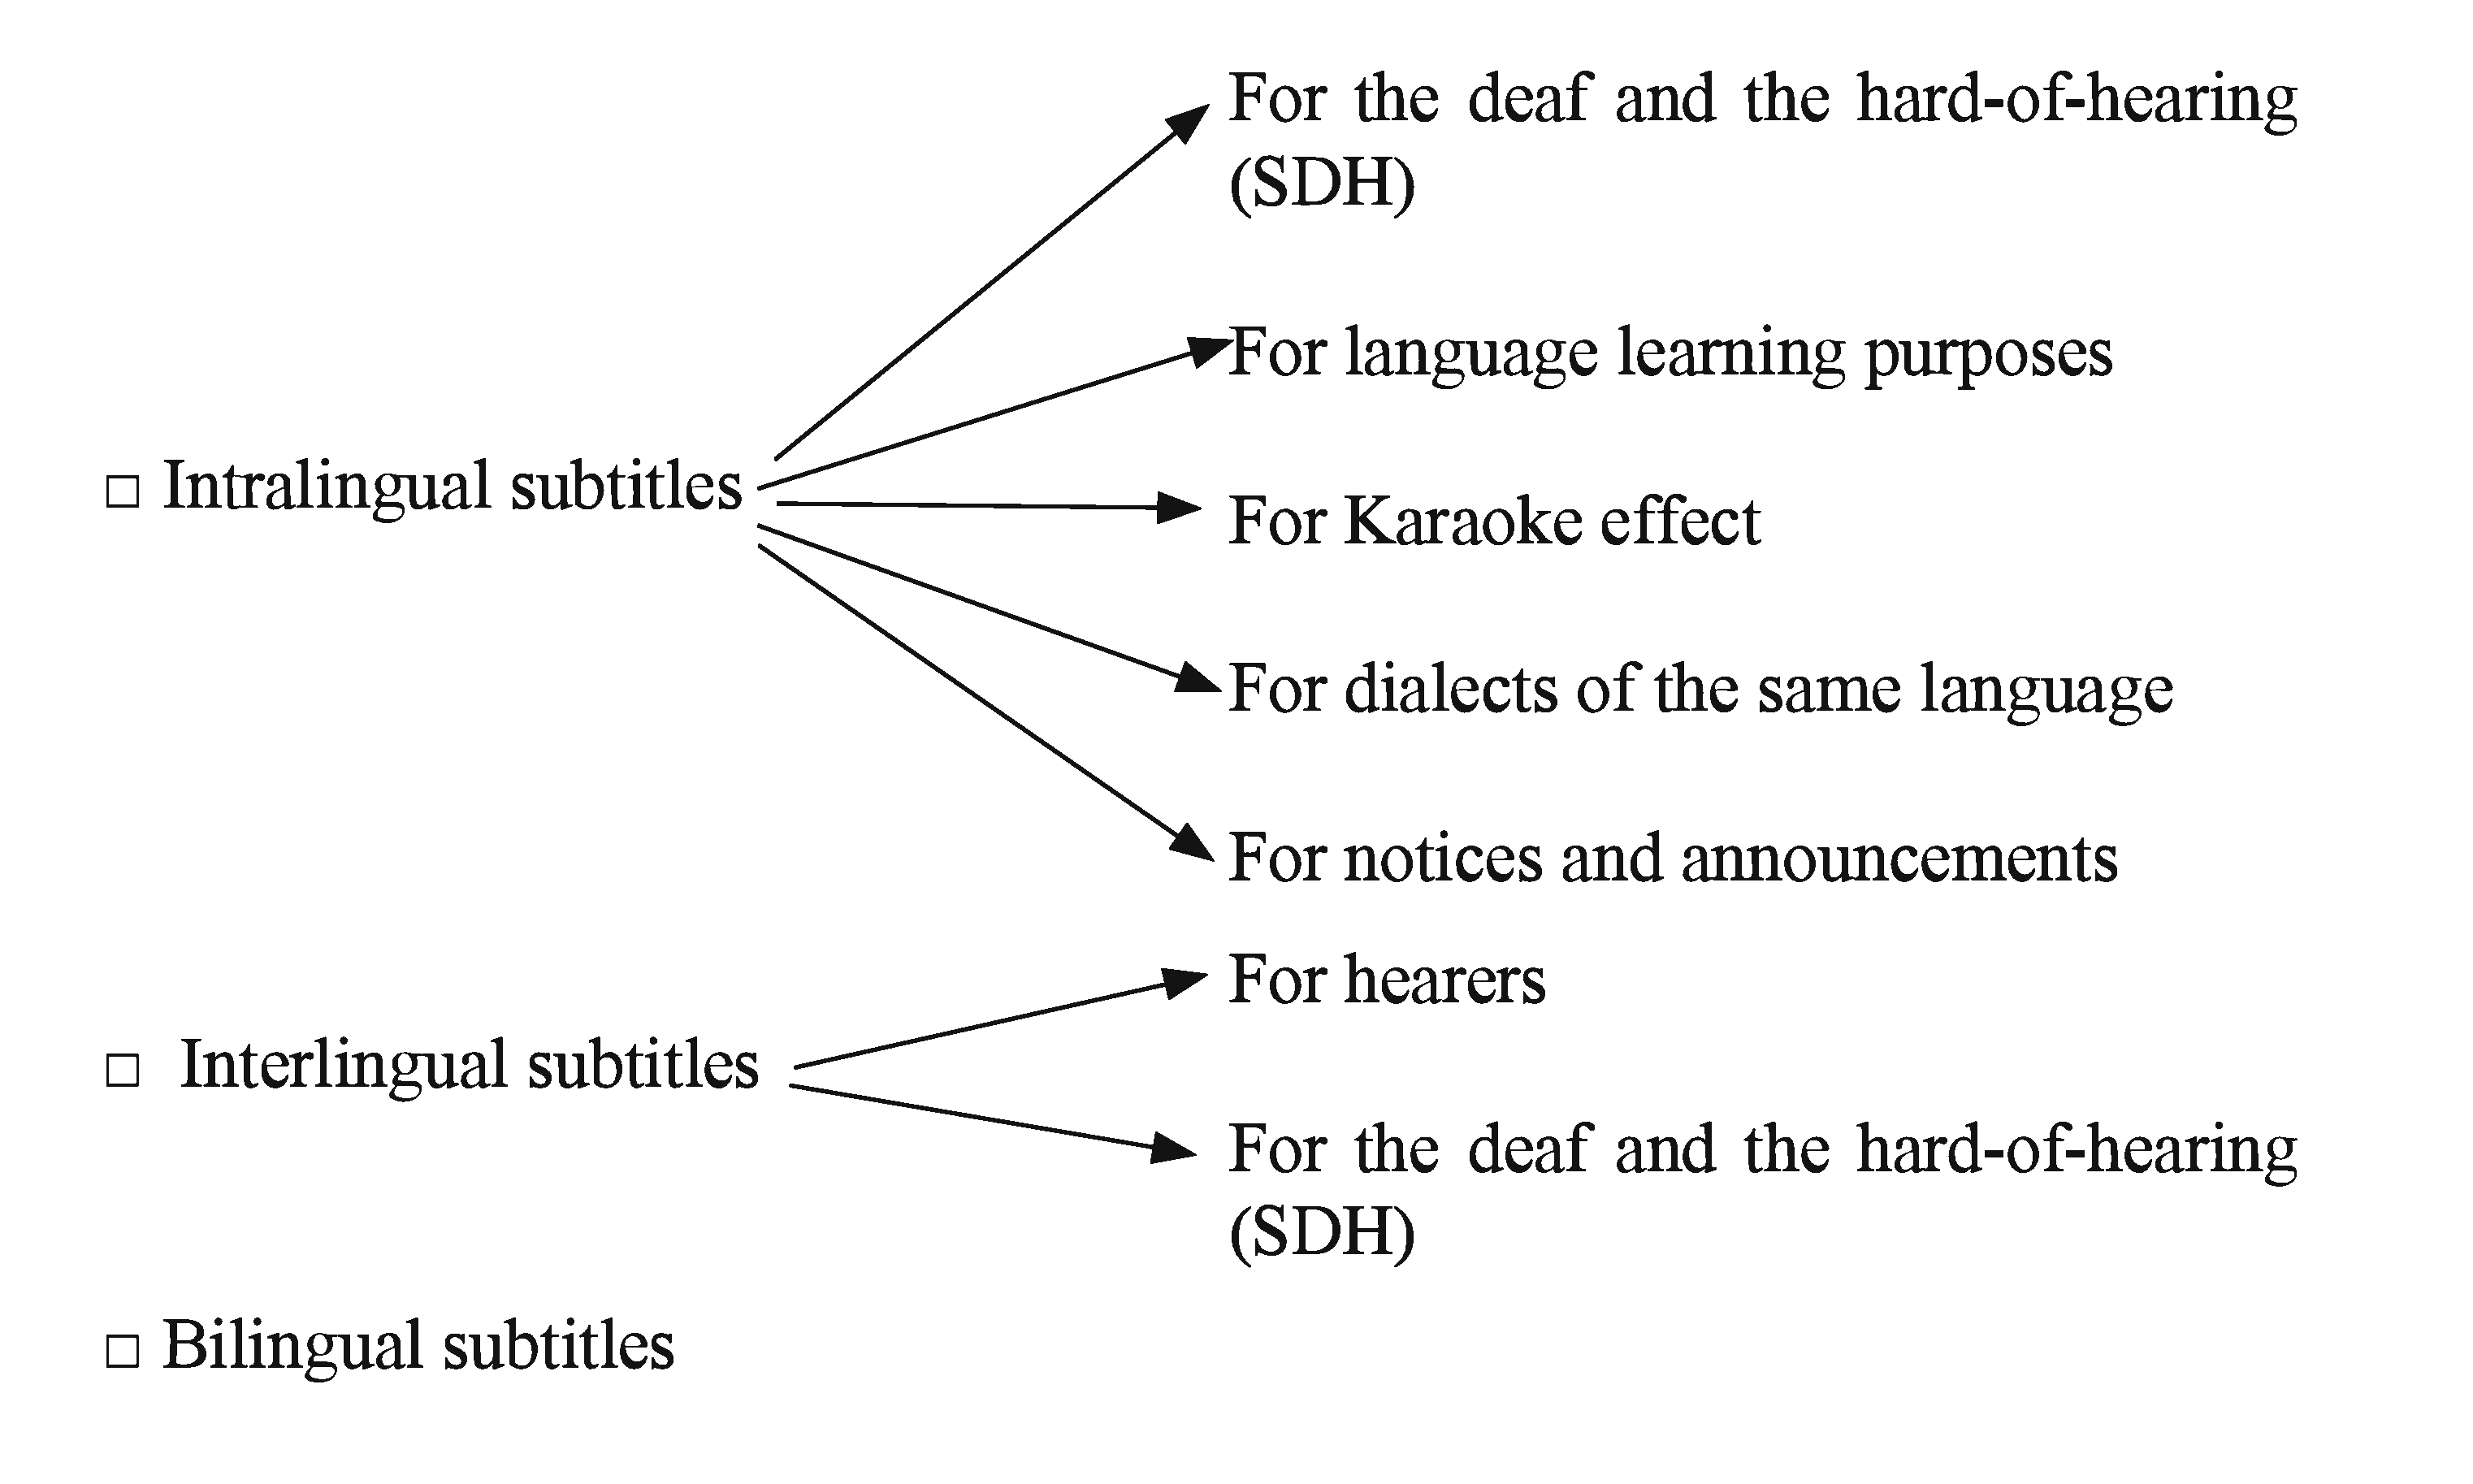
\includegraphics[width=\textwidth]{Picture1.pdf}
\caption{Classifications of subtitles based on linguistic dimension.}
\source{\cite[p. 14]{diaz-cintas__2007}.}
\label{fig:fig1}
\end{minipage}
\end{figure}

When considering the available time for preparation, subtitles can be
categorised into various types. \textcite{diaz-cintas__2007} classified them into pre-prepared subtitles and live or
real-time subtitles, as \Cref{fig:fig2} shows.

\begin{figure}[htbp]
\centering
\begin{minipage}{.7\textwidth}
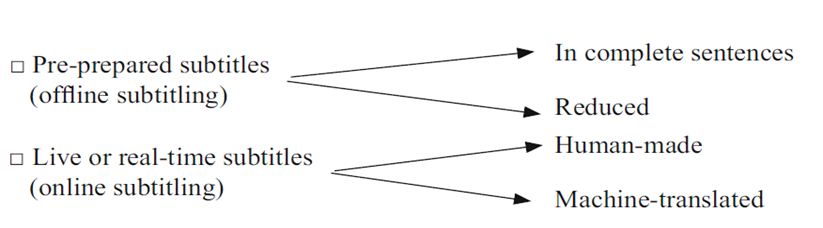
\includegraphics[width=\textwidth]{Picture2.png}
\caption{Classifications of subtitles based on time available for preparation.}
\source{\cite[p. 19]{diaz-cintas__2007}.}
\label{fig:fig2}
\end{minipage}
\end{figure}

Recent developments in voice and speech recognition have made possible
the appearance of respeaking as a practice to subtitle programmes that
are broadcast (semi/real) live, such as the news or sports \cite{remael_audiovisual_2010}. 
Auto-generated subtitles usually depend on two main artificial
intelligence technologies: Automatic Speech Recognition and Machine
Translation. Automatic speech recognition (ASR) is a machine-based
method that independently decodes and transcribes oral speech
\cite{suvorov_automatic_2012}.

\textcite{dharmale_evaluation_2019} mention that
``Automatic Speech Recognition permits the machine to take out oral
contained from a speech signal and produce a text message by using
feature extraction and classification techniques.'' As part of Spoken
Language Translation, Machine Translation (MT) can be defined as the
subfield of computational linguistics concerned with using software in
translation across human languages \cite{almahasees_machine_2017}.
	
\subsubsection{AI-powered Subtitles}\label{subsubsec-AI-powered-Subtitles}

Through a detailed review of the relevant literature and a comprehensive
analysis of various forms of AI-powered subtitles, it has become
apparent that it is essential for academic research in AVT to
distinguish between these different types. Therefore, to align with our
research objectives and due to the insufficient literature available, a
classification system has been developed for AI-powered subtitles to
identify the subtitle types used in the study accurately.

Artificial Intelligence (AI) powered subtitles use machine learning
algorithms and natural language processing (NLP) techniques to generate
audio or video content subtitles. This approach involves using AI to
analyse the audio or video content, transcribe the spoken words, sign
language, or paralinguistic elements and generate accurate and
synchronised subtitles.

AI-powered subtitles can be categorised based on various factors. In
this study, the categorisation is based on two main factors, namely, the
used technology and the target language. \emph{The used technology}
refers to some technologies used in recent years. Some of these are
sound recognition (SR), automatic speech recognition (ASR), sign
language recognition (SLR), machine translation (MT), and others. These
technologies are all focused on language processing and understanding.
\emph{The target language,} where the process of generating subtitles
may be influenced by the target audience. For instance, social media
platforms in the Arab world tend to use MSA for subtitles, as it covers
a wide geographical area and avoids the time-consuming task of
generating subtitles for specific dialects. However, for automatic
speech recognition (ASR) subtitles, Facebook generates comprehensible
subtitles for the dialects that may contain orthographical errors,
mainly related to glottal stop variants in Arabic, and mixes them with
Alef or some phonetic-based errors like the one on the Egyptian dialect
where they tend to pronounce any voiceless dental fricative consonantal
sound \ipa{/θ/} as voiceless alveolar fricative \ipa{/s/}, and therefore, the model
generates the Arabic character \textlang{arabic}{س}, so \textlang{arabic}{سعلب} instead of
\textlang{arabic}{ثعلب}.

Drawing on the linguistic dimension classifications presented by
\cite{diaz-cintas__2007}, AI-generated subtitles can be
categorised as Intralingual AI-powered subtitles and Interlingual
AI-powered subtitles.

\emph{Intralingual AI-powered subtitles} are intralingual subtitles that
use different technologies to produce a written form within the same
language. These could be categorised as SR-based subtitles, ASR-based
subtitles, Semi-ASR subtitles, and SLR-based subtitles. \emph{SR-based
	subtitles} refer to subtitles generated using a combination of automatic
speech recognition and other sound recognition techniques. ASR is used
to transcribe spoken language into written text, while SR is used to
filter and extract relevant information from the audio signal, such as
noise, music, and non-speech elements. Combining these techniques can
improve the accuracy and quality of the generated subtitles, providing a
complete viewing experience for people such as the Deaf and Hard of
Hearing (DHH). YouTube excelled in this type of AI-powered subtitles,
adding a good description for the paralinguistic elements in their
auto-generated subtitles. \emph{ASR-based subtitles}, where the
spoken words in written form of an audio or video file are analysed and
transcribed. ASR subtitles have become a ubiquitous feature on social
media platforms such as Facebook, which generates these subtitles in
multiple languages and different dialects. In addition, several
platforms offer the service of auto-generated subtitles for videos for
content creators and companies (paid and unpaid), such as Amara and
Zubtitle. Without including any description for paralinguistic elements,
ASR-based subtitles are for hearing people, which helps them to
understand the spoken language better without semiotic or paralinguistic
elements, i.e., the transcription of the spoken words only. It helps
people understand language and dialects and follow along with the verbal
elements.

\emph{Semi-ASR subtitles} are generated using a combination of automatic
speech recognition (ASR) technology and manual human intervention. The
initial transcription is generated by an ASR system, and then a human
editor reviews and corrects the transcription to ensure accuracy and
readability. Vimeo and Veed.io offer the service of ASR subtitles and
enable users to edit these subtitles. \emph{SLR-based subtitles} are
generated based on SLR technology and translate sign language into a
written form. SignAll and SLAIT provide their clients with a system that
translates between sign language and written/spoken text in a way that
the system captures signed language using a system of four cameras. It
detects body movements and expressions to translate American sign
language to English written form and displays it on the screen. \Cref{fig:fig3}
illustrates the classifications of AI-powered subtitles.

\begin{figure}[htbp]
\centering
\begin{minipage}{.7\textwidth}
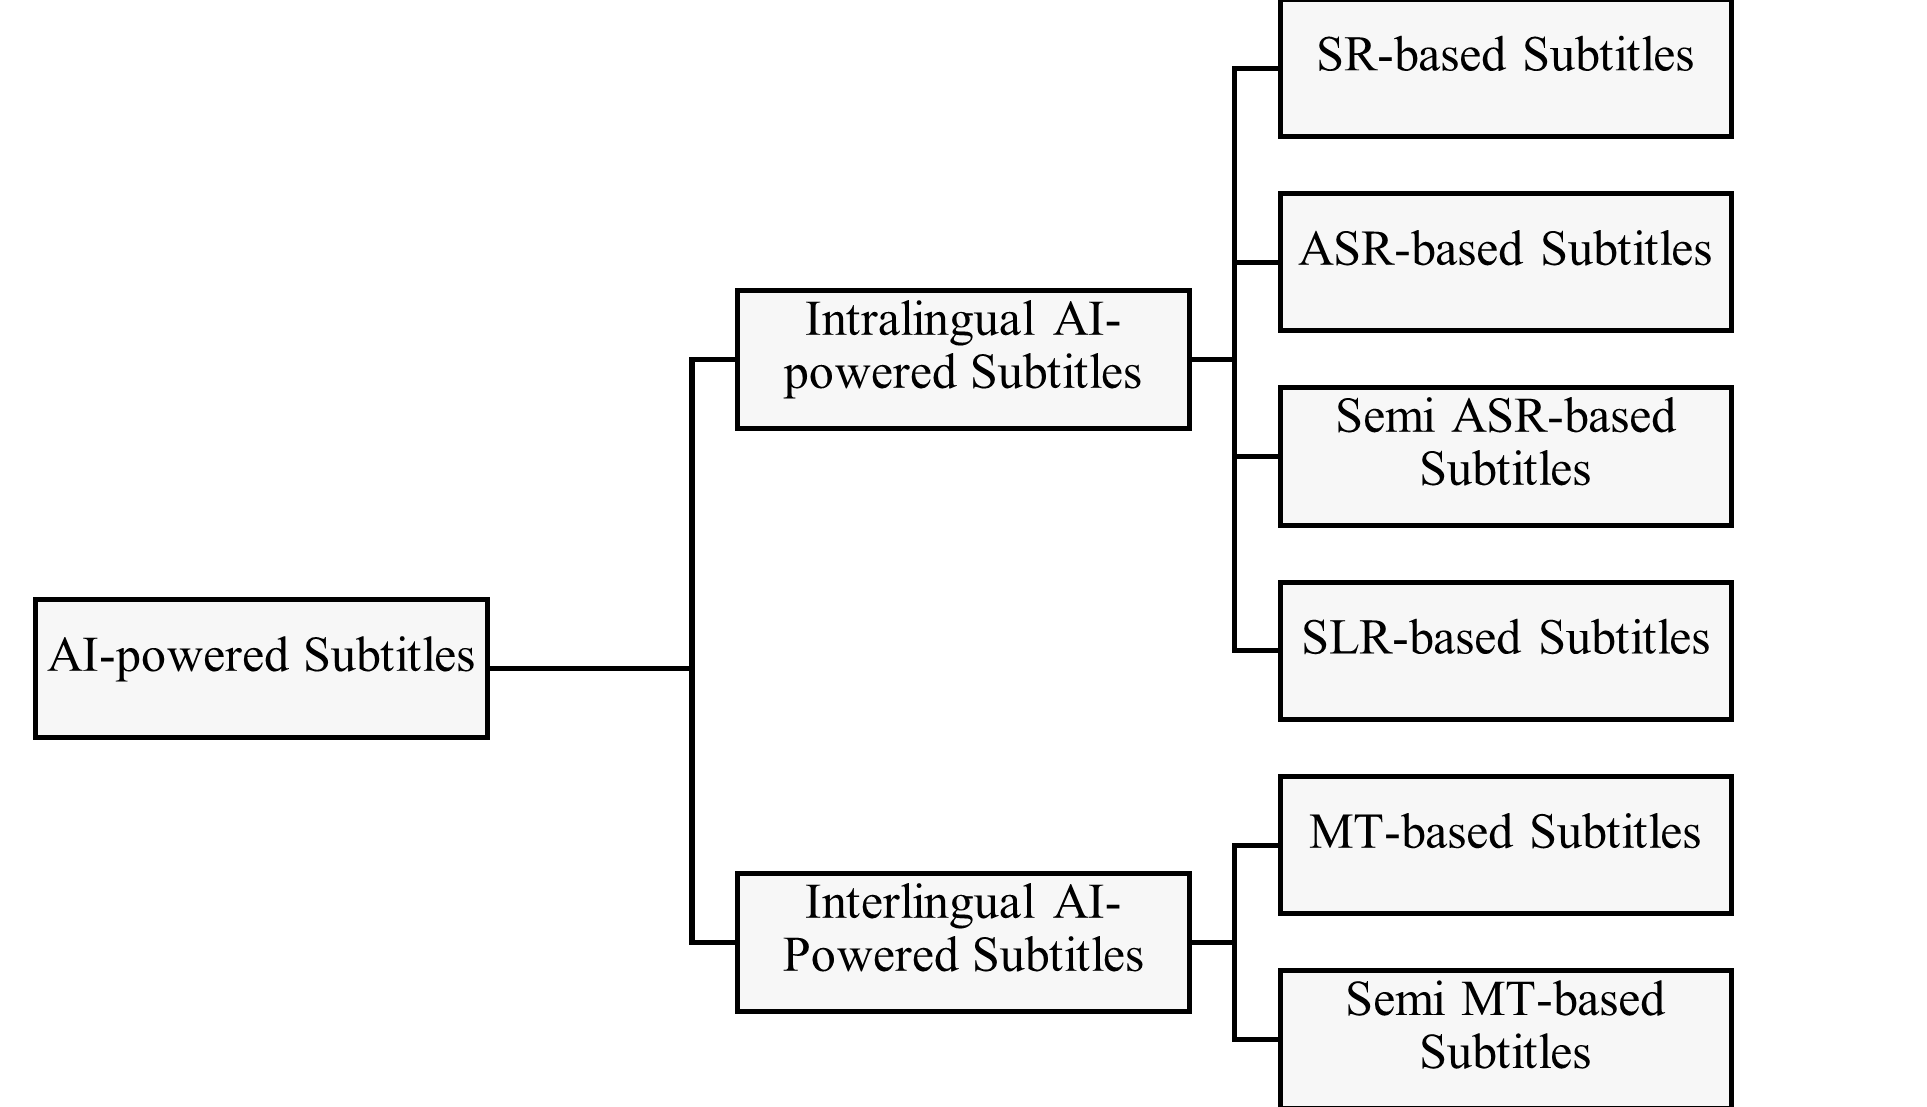
\includegraphics[width=\textwidth]{Picture3.png}
\caption{Classifications of Artificial Intelligence-Powered
	Subtitles.}
\source{Own Elaboration.}
\label{fig:fig3}
\end{minipage}
\end{figure}


\emph{Interlingual AI-powered subtitles} are interlingual subtitles that
use technologies to analyse a language's spoken content and produce a
written form in another language. These include MT-based subtitles and
Semi-MT-based subtitles. \emph{MT-based subtitles} are generated using
automated translation software rather than being translated by human
translators. This technology uses algorithms to automatically translate
spoken, written, or sight content from one language to another. On their
videos, Facebook added the feature of choosing the closed caption in
languages other than the video's original language. \emph{Semi-MT-based
subtitles} are the MT subtitles generated by the software, and a human
operator edits them to level up the accuracy, i.e., the post editor.
Using YouTube Studio for content creators enables them to edit captions
created automatically, generating a new caption track that includes
their revisions. The current study is focused on ASR-based subtitles and
MT-based subtitles.
	
\subsubsection{Arabic Language and Jordanian Arabic Dialect}\label{subsubsec-Arabic-Language-and-Jordanian-Arabic-Dialect}

Modern Standard Arabic is the language of written Arabic media,
\emph{e.g.}, newspapers, books, journals, street signs, and
advertisements. It is also the language of the majority of news
broadcasts on radio and television \cite{ryding_reference_2005}.
\textcite[p. 185]{sabir_brief_2014} stated that ``Arabic
has 28 consonants (including two semi-vowels) and six vowels (three
short vowels and three long vowels)''. As a common phenomenon,
diglossia in the Arab world is a normal situation where people speak and
shift between the standard language and their regional dialect.
Geographically speaking, Arabic is one of the most widely spoken
languages in the world, and its dialects are spoken in a continuous
stretch from western Iran through Mauritania and Morocco and from Oman
to northern Nigeria, despite the enormous deserts and sparsely populated
or uninhabited regions in between \cite{behnstedt_dialectology_2013}.

Arabic speakers speak a variety of mutually intelligible dialects that
differ in phonology, morphology, syntactic structure, lexical content,
geography, and social structure. However, they are rarely written;
therefore, there are no stable writing conventions \cite{maamouri_developing_2006}. In his conclusion,
\textcite{doughan_imaginaries_2017} stated that ``Jordanians
meta-pragmatically differentiate between two registers of Arabic in
Jordan: Urdunī (Jordanian) and Madanī (Urban)'' (p.103).

In the case of the city of Amman, \textcite[p. 325]{versteegh_encyclopedia_2006} pointed out that ``The new dialect primarily relies on elements
from the madanī (Urban) dialect as well as elements from the Jordanian
Bedouin dialect''. In conclusion, in Jordan, most media
productions are produced in the dialect that is spoken in Amman, which
is the urban dialect. Therefore, it is essential to focus on choosing
data spoken in this specific dialect in addition to MSA.

\subsection{Empirical Studies}\label{subsec-Empirical-Studies}
The field of automatic speech recognition (ASR) has seen an interest in
recent years in the field of natural language processing. Yet, it is
worth noting that ASR non-computational studies were lacking.

A systematic review by \textcite{alharbi_automatic_2021} summarised the most important topics of ASR published in the
last six years. published in the last six years. The study reported the
most applied datasets in recent ASR research, categorising the reviewed
articles based on three characteristics: domain problems, natural
language pre-processing, and device efficiency. The review identified
several challenges facing ASR, including speech capture issues,
hardware-related problems with microphones, and speech pre-processing
challenges such as dialect diversity and pronunciation problems.
Finally, the study suggested future research directions for improving
ASR systems.

Reviewing some specific linguistic phenomena in ASR systems has
attracted much attention from research teams. In their experiment,
\textcite{mustafa_code-switching_2022} measured
code-switching (CS) in automatic speech recognition (ASR) systems. CS is
when speech has two or more languages within an utterance. The research
has identified 274 papers and selected 42 experimental papers for review
covering many well-resourced and under-resourced languages and
techniques to recognise CS in ASR systems, such as mapping, combining,
and merging the phone sets of the languages experimented with and
examined the performance of those techniques. The study found a
significant variation in the performance of CS experimental papers in
terms of word error rate (WER), indicating the inconsistency in the
existing ASR systems' ability to handle unexpected pronunciation changes
when languages are mixed.

Likewise, \textcite{sawakare2015}
discussed the techniques used in various stages of speech recognition,
classifying speech recognition systems based on utterance types,
vocabulary sizes, and speaker modes used. They noted that feature
extraction is essential in separating relevant from irrelevant
information and distinguishing one speech from another. Moreover, they
concluded that feature extraction played a significant role in improving
speech recognition system accuracy.

However, while many studies focused on the NLP field,
\textcite{guskaroska_asr_2019} examined the usefulness of
mobile-assisted ASR dictation systems for enhancing vowel pronunciation
among Macedonian EFL learners. The study utilised a mixed-methods
approach, which included pre-test and post-test recordings to measure
accuracy gains, a comparison of ASR written output to humans, and an
analysis of learners' attitudes towards ASR through Facebook posts. The
findings revealed that the experimental group (Non-Native English
Speakers) had improved accuracy while the control group (Native English
Speakers) did not. In addition, learners generally had positive
attitudes toward ASR. The study suggested incorporating mobile-assisted
ASR in EFL classrooms with careful teacher guidance and structured
practice using individual words.

Some researchers in the auto-generated subtitling field are concerned
about paralinguistic components being visible in the subtitles. An
experimental study guided by \textcite{schlippe_visualizing_2020} evaluated a new method called WaveFont, which diversifies
fonts in video captions based on voice characteristics such as loudness,
speed, and pauses. The goal was to test this new method specifically for
Arabic viewers and to compare it to traditional captions. The results
showed that WaveFont is comprehensible and accepted by most people,
including deaf and hard of hearing and normal-hearing viewers. The study
suggested that this technology can revolutionise how captions and
subtitles are presented, with potential applications in various fields
such as video-on-demand, TV, social media, live broadcasts, and public
places.

\textcite{liao_improving_2023} introduced a new
method which is the ASR post-processing for readability (APR) task. The
goal of this task is to enhance ASR output by correcting grammatical
mistakes, disfluency and making it more readable for humans. They used
the Grammatical Error Correction datasets as their corpus by using TTS
and ASR systems. Also, they adapt and develop evaluation metrics from
related tasks. Their method proved to be effective since the human
evaluation and case study further revealed the ability of the proposed
model to improve the readability of ASR transcripts.

In their article, \textcite{pucci_towards_2023} addressed some
of the opportunities and challenges offered by automatic speech
recognition (ASR) systems. They discussed both the advantageous aspects
and challenges presented by ASR systems. The researcher pointed out that
ASR technology is a valuable tool for presenting information in a
multimodal manner, supporting inclusivity and communication improvement.
However, they mentioned that further refinement of this technology is
required before incorporating it into universally designed environments.

When it comes to Machine translation, several publications have appeared
in recent years documenting the level of accuracy of MT software, making
the studies in the non-computational fields, specifically AVT studies,
richer and wider.

\textcite{al_mahasees_analysing_2021} conducted a comparative
evaluation of the performance of three machine translation (MT) systems
for Arabic: Sakhr, Google Translate, and Microsoft Translator. The study
analysed the output of the three systems on both holistic analysis and
error analysis (EA) scales to provide constructive feedback about their
capacity. In addition, the study ranked the three systems' performance
based on their adequacy, fluency scales, and error categories, including
orthography, lexis, grammar, and semantic errors. Google Translate
achieved the best overall performance, followed by Microsoft Translator
and Sakhr.

Adopting a user-centric approach, \textcite{xie_comparative_2022}
compared machine-translated subtitles on Bilibili (MTS-B) with those on
YouTube (MTS-Y) and investigated the relationship between the quality,
users' comprehension, and attitude towards machine-translated subtitles.
The study found that quality had little impact on users' comprehension
of the videos. However, accuracy had a significant effect on users'
attitudes toward the quality of the translation. Participants had a
better attitude towards MTS-Y as it performed better in accuracy. The
study also found that MTS-Y performed better in grammar and spelling,
while MTS-B showed cleaner and simpler subtitles. Overall, most
participants could understand the contents of the video through the
machine-translated subtitles.

Moreover, \textcite{almahasees_facebook_2020}
investigated the use of Facebook Translation Service (FTS) as a source
of information during the COVID-19 lockdown in Jordan. The study found
that Facebook and FTS became significant sources of information during
the crisis, with 62.2\% of participants considering Facebook as their
primary source of information regarding COVID-19. Additionally, 87.1\%
of participants activated FTS, with 87.3\% using FTS to translate
English Facebook posts into Arabic. However, the majority found that FTS
committed minor errors in terms of adequacy and fluency. The study
suggested that health officials should create Facebook profiles with a
blue tick for medical information during crises. In addition, medical
specialists and translation scholars should evaluate FTS's ability to
render COVID-19 medical posts fluently and adequately in Arabic.

As it is shown, for several years, different scholars have investigated
ASR and MT from a computational linguistics perspective. However, to our
knowledge, an evaluation of the ASR systems from a linguistic
perspective is not common. This work is the first of its type, making
the evaluation and analysis of AI-powered subtitles complex.

\section{Methodology}\label{methodology}
	
This section presents an overview of the methodology used in the study.
It includes details about the sample and data collection process. The
study employs a combination of quantitative and qualitative approaches.
The procedures followed in the study are also summarised at the end of
this section.


\subsection{Selected Data}\label{subsec-Selected-Data}
\subsubsection{ASR-based subtitles}\label{subsubsec-ASR-based-subtitles}

To ensure the investigation's success, the selection of videos is based
on various factors that mainly surround the utterances, which will be
analysed and transcribed by the model. These challenging factors could
be related to the speakers' voices, such as voice quality, gender, age,
breath, clicks, pauses, stress, overlapping, mumbles, and prosody. Other
factors are related to the surrounding environment being part of the
acoustic signal, such as background noise and music. Therefore, the
chosen video is selected purposefully. The video is a Radio/TV show that
is recorded with high-quality microphones and published during the year
of the study. In the video, two Jordanian broadcasters use the dialect
of Amman to talk about the etiquette of meals in the month of Ramadan,
where they code-switch/mix, laugh, and speak fast and slow in their
show. The video to be tested is shown below in \Cref{tbl01}.

\begin{table}[htbp]
\centering
\begin{threeparttable}
\caption{Selected video for the investigation of the study.}
\label{tbl01}
\begin{tabular}{lp{5.5cm}p{5.5cm}}
Video Type & Link & Justifications \\
\midrule
Radio/TV shows & \url{https://www.youtube.com/watch?v=MeDi-77lQ24} & Gender, Code Switching, Mumbling, Overlapping chatter. \\
\bottomrule
\end{tabular}
\source{Own elaboration.}
\end{threeparttable}
\end{table}

The website that will be tested for the ASR investigation is
\href{http://www.veed.io/}{www.veed.io}. On
LinkedIn\footnote{Veed.io Linkedin page:
\url{https://www.linkedin.com/company/veedhq}.}, Veed.io define themselves as
``An AI-powered online video editing platform that makes creating videos
easy and accessible to everyone''. This website provides content
creators and businesses with tools that can help them edit their videos
and add automatic subtitles in many languages and dialects. In the year
of this study, before generating the subtitles, the user should select
which language is spoken in the video. Among the choices, the Arabic
language is available, and they can choose one of the following
dialects: Jordanian, Palestinian, Lebanese, Iraqi, Saudi, Bahraini,
Qatari, Kuwaiti, Omani, Egyptian, Tunisian, Algerian, and Moroccan.

The analysis will mainly focus on the linguistic aspects by categorising
the errors into two main types. Errors that did not significantly affect
the comprehension of the text were given a value of 0.5, while errors
that affected the comprehension of the subtitles were given a value of
1. \Cref{tbl02} shows the categorisation of these errors based on their
types.
	
\begin{table}[htbp]
\centering
\begin{threeparttable}
\caption{Categorisation of errors based on their type.}
\label{tbl02}
\begin{tabular}{lllll}
\multicolumn{5}{c}{0.5 Errors} \\
	Type/Category & 1 & 2 & 3 & 4 \\
\midrule
Deletions & Affixes & Interjections & Overlapping & Vowel length \\
Substitutions & Affixes & Interjections & Overlapping & Pronouns \\
Insertions & Affixes \\
&&&&\\
\multicolumn{5}{c}{1.0 Errors} \\
Type/Category & 1 & 2 & 3 & 4 \\
\midrule
Deletions & Nouns & Verbs & Function words & Foreign words \\
Substitutions & Nouns & Verbs & Function words & Foreign words \\
Insertions & Nouns & Verbs & Function words \\
\bottomrule
\end{tabular}
\source{Own elaboration.}
\end{threeparttable}
\end{table}
	
	


\subsection{Data Analysis Approaches}\label{subsec-Data-Analysis-Approaches}
	
The study contains quantitative and qualitative parts. This combined
approach can result in a more thorough and nuanced exploration of the
analysis.


\subsubsection{Qualitative method}\label{subsubsec-Qualitative-method}

Here, the analysis investigates the errors using a manual evaluation
based on linguistic and lexical factors by comparing the generated
transcription to the audible utterances. The study discusses the errors
categorised into two values (0.5) and (1.0). Errors of Affixes, vowel
length, and overlapping are given a 0.5 value, while errors of nouns,
verbs, foreign words, and function words that are not affixed are given
a 1.0 value.


\subsubsection{Quantitative method}\label{subsubsec-Quatitative-method}

Word Error Rate (WER) is calculated. \textbf{WER} is a metric that
measures the difference between the transcript generated by an ASR
system and the actual transcript. Here, we calculate the percentage of
words that were incorrectly transcribed by the ASR system. A lower WER
indicates a higher-quality transcript.


\subsection{Study Procedures}\label{subsec-Study-Procedures}

The procedures that are followed for the investigation of the
\emph{ASR-based subtitles} are as follows.


\begin{itemize}
\item \textbf{In the qualitative part:}
	\begin{enumerate}
	\item The video is transcribed manually using Arabic Abjads in correct non-diacritised Arabic orthography (Without \emph{ḥarakāt}).
	\item The transcription is divided into segments in an Excel sheet.
	\item The transcription is on one sheet, where this sheet represents the data and details for the website.
	\item The video is uploaded to the testing website. 
	\item The website generates auto-generated subtitles.
	\item The generated transcription is extracted to txt. file, which ensures that the only data there is textual.
	\item The transcription is segmented into a column in one sheet.
	\item The errors are detected and analysed in the analysis section.
	\end{enumerate}
\item \textbf{In the quantitative part:}
	\begin{enumerate}
	\item The video is transcribed manually using Arabic Abjads in correct
	non-diacritised orthography and is considered to be the reference
	transcript.
	\item The transcript is divided into segments on an Excel sheet.
	\item The transcript is on one sheet, where the sheet represents the data
	and details for the testing website.
	\item The video is uploaded to the testing website.
	\item The website generates subtitles.
	\item The ASR-generated transcript (subtitles) is extracted to txt. file.
	This ensures that the only data there is textual data.
	\item The reference and ASR-generated transcripts are aligned. This
	determines which words in the ASR-generated transcript correspond to
	which words in the reference transcript.
	\item WER is calculated: The calculations of WER is computed using the
	following formula using Excel (Shah \emph{et al}., 2022):
	\end{enumerate}

\begin{equation}\nonumber
    \text{WER} = (S + D + I) / N
\end{equation}

$S =$ Number of substitutions (words in the ASR-generated transcript that differ from the corresponding words in the reference transcript).

$D =$ Number of deletions (i.e., words in the reference transcript that are missing from the ASR-generated transcript)

$I =$ Number of insertions (i.e., words in the ASR-generated transcript that are not present in the reference transcript)

$N =$ The total number of words in the reference transcript.

	\begin{enumerate}[resume]
	\item WER is interpreted using a percentage. A lower value indicates better
	accuracy. For example, a WER of 5\% means that 5 out of every 100
	words in the ASR-generated transcript are incorrect.
	\end{enumerate}

\end{itemize}

\section{Findings and Discussion}\label{sec-findings-and-discussion}

\subsection{Qualitative Analysis}\label{subsec-Qualitative-Analysis}

\subsubsection{Deletions}\label{subsubsec-Deletions}

This section analyses the deletion errors. First, it discusses errors
with 0.5, including affixes, interjections, overlapping, and vowel
length. Second, it discusses errors with a 1.0 value, including nouns,
verbs, function words, and foreign words. \Cref{tbl03} below shows some
examples of 0.5 deletion errors.
	
\begin{table}[htbp]
\small
\centering
\begin{threeparttable}
	\caption{Examples of 0.5 deletion errors in the ASR-based subtitles.}
	\label{tbl03}
	%\renewcommand{\arraystretch}{1.35}
	%\begin{longtable}[]{@{}
	\begin{tabular}{@{}
			>{\raggedright\arraybackslash}p{(\columnwidth - 12\tabcolsep) * \real{0.0700}}
			>{\raggedright\arraybackslash}p{(\columnwidth - 12\tabcolsep) * \real{0.1500}}
			>{\raggedright\arraybackslash}p{(\columnwidth - 12\tabcolsep) * \real{0.1200}}
			>{\raggedright\arraybackslash}p{(\columnwidth - 12\tabcolsep) * \real{0.1356}}
			>{\raggedright\arraybackslash}p{(\columnwidth - 12\tabcolsep) * \real{0.0008}}
			>{\raggedright\arraybackslash}p{(\columnwidth - 12\tabcolsep) * \real{0.1855}}
			>{\raggedright\arraybackslash}p{(\columnwidth - 12\tabcolsep) * \real{0.1356}}@{}}
		\noalign{}
		\begin{minipage}[b]{\linewidth}\raggedright
			No.
		\end{minipage} &
		\multicolumn{2}{>{\raggedright\arraybackslash}p{(\columnwidth - 12\tabcolsep) * \real{0.4237} + 2\tabcolsep}}{%
			\begin{minipage}[b]{\linewidth}\raggedright
				Error Type
		\end{minipage}} &
		\multicolumn{2}{>{\raggedright\arraybackslash}p{(\columnwidth - 12\tabcolsep) * \real{0.1365} + 2\tabcolsep}}{%
			\begin{minipage}[b]{\linewidth}\raggedright
				IPA (JA)
		\end{minipage}} & 
		\begin{minipage}[b]{\linewidth}\raggedright
			Utterance
		\end{minipage} & 
		\begin{minipage}[b]{\linewidth}\raggedright
			ASR subtitle
		\end{minipage} \\
		\toprule
		%\endhead
		
		
		\multicolumn{1}{c}{1} & Affix & \multicolumn{1}{|l}{Present Progressive Particle} &
		\multicolumn{2}{>{\raggedright\arraybackslash}p{(\columnwidth - 12\tabcolsep) * \real{0.1365} + 2\tabcolsep}}{\ipa{%
				/b/, /bi/}} & \textlang{arabic}{بتوصل، بتكون} & \textlang{arabic}{توصل، تكون} \\
		
		\multicolumn{1}{c}{2} & Affix & \multicolumn{1}{|l}{Coordinating Conjunction} &
		\multicolumn{2}{>{\raggedright\arraybackslash}p{(\columnwidth - 12\tabcolsep) * \real{0.1365} + 2\tabcolsep}}{\ipa{%
				/w/, /wa/}} & \textlang{arabic}{و} & X \\
		
		\multicolumn{1}{c}{3} & Affix & \multicolumn{1}{|l}{Definite article} &
		\multicolumn{2}{>{\raggedright\arraybackslash}p{(\columnwidth - 12\tabcolsep) * \real{0.1365} + 2\tabcolsep}}{\ipa{%
				/ʔal/ , /ʔa/}} & \textlang{arabic}{ال ال ال ، الست ، التحية} & X \textlang{arabic}{، ست، تحية} \\
		
		\multicolumn{1}{c}{4} &
		\multicolumn{2}{>{\raggedright\arraybackslash}p{(\columnwidth - 12\tabcolsep) * \real{0.4237} + 2\tabcolsep}}{%
			Third singular masculine pronoun (Object)} &
		\multicolumn{2}{>{\raggedright\arraybackslash}p{(\columnwidth - 12\tabcolsep) * \real{0.1365} + 2\tabcolsep}}{\ipa{%
				hi}} & \textlang{arabic}{فيه} & \textlang{arabic}{في} \\
		
		\multicolumn{1}{c}{5} &
		\multicolumn{2}{>{\raggedright\arraybackslash}p{(\columnwidth - 12\tabcolsep) * \real{0.4237} + 2\tabcolsep}}{%
			Coordinating Conjunction/ Connective particle} &
		\multicolumn{2}{>{\raggedright\arraybackslash}p{(\columnwidth - 12\tabcolsep) * \real{0.1365} + 2\tabcolsep}}{\ipa{%
				/fa/}} & \textlang{arabic}{فانت، فبيقولك} & \textlang{arabic}{انت، بقولك} \\
		
		\multicolumn{1}{c}{6} &
		\multicolumn{2}{>{\raggedright\arraybackslash}p{(\columnwidth - 12\tabcolsep) * \real{0.4237} + 2\tabcolsep}}{%
			Preposition} &
		\multicolumn{2}{>{\raggedright\arraybackslash}p{(\columnwidth - 12\tabcolsep) * \real{0.1365} + 2\tabcolsep}}{\ipa{%
				/b/, /bi/}} & \textlang{arabic}{بأريحية، بالموضوع} & \textlang{arabic}{اريحيه، الموضوع} \\
		
		\multicolumn{1}{c}{7} &
		\multicolumn{2}{>{\raggedright\arraybackslash}p{(\columnwidth - 12\tabcolsep) * \real{0.4237} + 2\tabcolsep}}{%
			Preposition} &
		\multicolumn{2}{>{\raggedright\arraybackslash}p{(\columnwidth - 12\tabcolsep) * \real{0.1365} + 2\tabcolsep}}{\ipa{%
				\ipa{/la/}, \ipa{/li/}}} & \textlang{arabic}{للأشخاص، لقضية} & \textlang{arabic}{الأشخاص، قضيه} \\
		
		\multicolumn{1}{c}{8} &
		\multicolumn{2}{>{\raggedright\arraybackslash}p{(\columnwidth - 12\tabcolsep) * \real{0.4237} + 2\tabcolsep}}{%
			Preposition} &
		\multicolumn{2}{>{\raggedright\arraybackslash}p{(\columnwidth - 12\tabcolsep) * \real{0.1365} + 2\tabcolsep}}{\ipa{%
				/ʕa/}} & \textlang{arabic}{عأساس} & \textlang{arabic}{أساس} \\
		
		\multicolumn{1}{c}{9} &
		\multicolumn{2}{>{\raggedright\arraybackslash}p{(\columnwidth - 12\tabcolsep) * \real{0.4237} + 2\tabcolsep}}{%
			Suffix of singular feminine gender} &
		\multicolumn{2}{>{\raggedright\arraybackslash}p{(\columnwidth - 12\tabcolsep) * \real{0.1365} + 2\tabcolsep}}{\ipa{%
				/a/}} & \textlang{arabic}{الزايدة} & \textlang{arabic}{زايد} \\
		
		\multicolumn{1}{c}{10} &
		\multicolumn{2}{>{\raggedright\arraybackslash}p{(\columnwidth - 12\tabcolsep) * \real{0.4237} + 2\tabcolsep}}{%
			Suffix of plural feminine gender} &
		\multicolumn{2}{>{\raggedright\arraybackslash}p{(\columnwidth - 12\tabcolsep) * \real{0.1365} + 2\tabcolsep}}{\ipa{%
				/aːt/}} & \textlang{arabic}{وشربات} & \textlang{arabic}{وشربا} \\
		
		\multicolumn{1}{c}{11} &
		\multicolumn{2}{>{\raggedright\arraybackslash}p{(\columnwidth - 12\tabcolsep) * \real{0.4237} + 2\tabcolsep}}{%
			Imperfective second person, feminine, singular prefix} &
		\multicolumn{2}{>{\raggedright\arraybackslash}p{(\columnwidth - 12\tabcolsep) * \real{0.1365} + 2\tabcolsep}}{\ipa{%
				/t/}} & \textlang{arabic}{تحاولي} & \textlang{arabic}{حاولي} \\
		
		\multicolumn{1}{c}{12} &
		\multicolumn{2}{>{\raggedright\arraybackslash}p{(\columnwidth - 12\tabcolsep) * \real{0.4237} + 2\tabcolsep}}{%
			Imperfective second person, masculine, singular prefix} &
		\multicolumn{2}{>{\raggedright\arraybackslash}p{(\columnwidth - 12\tabcolsep) * \real{0.1365} + 2\tabcolsep}}{\ipa{%
				/ti/}} & \textlang{arabic}{تكسر} & \textlang{arabic}{كسر} \\
		
		\multicolumn{1}{c}{13} &
		\multicolumn{2}{>{\raggedright\arraybackslash}p{(\columnwidth - 12\tabcolsep) * \real{0.4237} + 2\tabcolsep}}{%
			Imperfective third person, masculine, singular prefix.} &
		\multicolumn{2}{>{\raggedright\arraybackslash}p{(\columnwidth - 12\tabcolsep) * \real{0.1365} + 2\tabcolsep}}{\ipa{%
				/j/}} & \textlang{arabic}{بيشوفك} & \textlang{arabic}{بشوفك} \\
		
		\multicolumn{1}{c}{14} &
		\multicolumn{2}{>{\raggedright\arraybackslash}p{(\columnwidth - 12\tabcolsep) * \real{0.4237} + 2\tabcolsep}}{%
			Imperfective third person, masculine, plural prefix.} &
		\multicolumn{2}{>{\raggedright\arraybackslash}p{(\columnwidth - 12\tabcolsep) * \real{0.1365} + 2\tabcolsep}}{\ipa{%
				/j/}} & \textlang{arabic}{بيساعدوها} & \textlang{arabic}{بساعدها} \\
		
		\multicolumn{1}{c}{15} &
		\multicolumn{2}{>{\raggedright\arraybackslash}p{(\columnwidth - 12\tabcolsep) * \real{0.4237} + 2\tabcolsep}}{%
			Imperfective second person, masculine, singular prefix} &
		\multicolumn{2}{>{\raggedright\arraybackslash}p{(\columnwidth - 12\tabcolsep) * \real{0.1365} + 2\tabcolsep}}{\ipa{%
				/t/}} & \textlang{arabic}{بتحبها} & \textlang{arabic}{بحبها} \\
		
		\multicolumn{1}{c}{16} &
		\multicolumn{2}{>{\raggedright\arraybackslash}p{(\columnwidth - 12\tabcolsep) * \real{0.4237} + 2\tabcolsep}}{%
			Imperfective first person, masculine, plural prefix} &
		\multicolumn{2}{>{\raggedright\arraybackslash}p{(\columnwidth - 12\tabcolsep) * \real{0.1365} + 2\tabcolsep}}{\ipa{%
				/na/}} & \textlang{arabic}{بنطلب} & \textlang{arabic}{بطلب} \\
		
		\multicolumn{1}{c}{17} &
		\multicolumn{2}{>{\raggedright\arraybackslash}p{(\columnwidth - 12\tabcolsep) * \real{0.4237} + 2\tabcolsep}}{%
			Accusative case marker (Nunation)} &
		\multicolumn{2}{>{\raggedright\arraybackslash}p{(\columnwidth - 12\tabcolsep) * \real{0.1365} + 2\tabcolsep}}{\ipa{%
				/an/}} & \textlang{arabic}{مثلا} & \textlang{arabic}{مثل} \\
		
		\multicolumn{1}{c}{18} &
		\multicolumn{2}{>{\raggedright\arraybackslash}p{(\columnwidth - 12\tabcolsep) * \real{0.4237} + 2\tabcolsep}}{%
			Interjection} &
		\multicolumn{2}{>{\raggedright\arraybackslash}p{(\columnwidth - 12\tabcolsep) * \real{0.1365} + 2\tabcolsep}}{%
		    \ipa{/ʔa\textbar{} ʔa /}} & \textlang{arabic}{آه' آه} & X \\
		
		\multicolumn{1}{c}{19} &
		\multicolumn{2}{>{\raggedright\arraybackslash}p{(\columnwidth - 12\tabcolsep) * \real{0.4237} + 2\tabcolsep}}{%
			Interjection} &
		\multicolumn{2}{>{\raggedright\arraybackslash}p{(\columnwidth - 12\tabcolsep) * \real{0.1365} + 2\tabcolsep}}{\ipa{%
				/ʔe/}} & \textlang{arabic}{أي} & X \\
		
		\multicolumn{1}{c}{20} &
		\multicolumn{2}{>{\raggedright\arraybackslash}p{(\columnwidth - 12\tabcolsep) * \real{0.4237} + 2\tabcolsep}}{%
			Interjection} &
		\multicolumn{2}{>{\raggedright\arraybackslash}p{(\columnwidth - 12\tabcolsep) * \real{0.1365} + 2\tabcolsep}}{\ipa{%
				/ʔam/}} & \textlang{arabic}{أمم} & X \\
		
		\multicolumn{1}{c}{21} &
		\multicolumn{2}{>{\raggedright\arraybackslash}p{(\columnwidth - 12\tabcolsep) * \real{0.4237} + 2\tabcolsep}}{%
			Overlapping} &\ipa{ / ˈʔak.tar ˈmen ˈsit.tˤaˤʕ.ʃar ˈsaː.ʕit ˈsˤjaːm/} &
		\multicolumn{2}{>{\raggedright\arraybackslash}p{(\columnwidth - 12\tabcolsep) * \real{0.1863} + 2\tabcolsep}}{%
			\textlang{arabic}{(هدول أصعب خمس دقايق) أكتر من ستطاشر ساعة صيام}} & \textlang{arabic}{(هدول أصعب
			
			خمس دقايق)} \\
		
		\multicolumn{1}{c}{\multirow{2}{*}{22}} &
		\multicolumn{2}{>{\raggedright\arraybackslash}p{(\columnwidth - 12\tabcolsep) * \real{0.4237} + 2\tabcolsep}}{%
			\multirow{2}{=}{Overlapping}} & \ipa{/ˈ tˤaj·jib ˈ jal·laː/} &
		\multicolumn{2}{>{\raggedright\arraybackslash}p{(\columnwidth - 12\tabcolsep) * \real{0.1863} + 2\tabcolsep}}{%
			\multirow{2}{=}{\textlang{arabic}{طيب يلا (أنا برجع الصحون) بس اكتر من هيك}}} &
		\multirow{2}{=}{\textlang{arabic}{(أنا برجع الصحون)}} \\
		
		\cline{4-4}
		
		& & & \ipa{/bas ˈʔak.tar min ˈheːk/} \\
		
		\multicolumn{1}{c}{23} &
		\multicolumn{2}{>{\raggedright\arraybackslash}p{(\columnwidth - 12\tabcolsep) * \real{0.4237} + 2\tabcolsep}}{%
			Vowel length} & \ipa{/mar.ˈraːt/} &
		\multicolumn{2}{>{\raggedright\arraybackslash}p{(\columnwidth - 12\tabcolsep) * \real{0.1863} + 2\tabcolsep}}{%
			\textlang{arabic}{مرات}} & \textlang{arabic}{مره} \\
		
		\multicolumn{1}{c}{24} &
		\multicolumn{2}{>{\raggedright\arraybackslash}p{(\columnwidth - 12\tabcolsep) * \real{0.4237} + 2\tabcolsep}}{%
			Vowel length} & \ipa{/ ˈʔaː.lat/} &
		\multicolumn{2}{>{\raggedright\arraybackslash}p{(\columnwidth - 12\tabcolsep) * \real{0.1863} + 2\tabcolsep}}{%
			\textlang{arabic}{قالت}} & \textlang{arabic}{قلت} \\
		
		\bottomrule
		%\end{longtable}
	\end{tabular}
	\source{Own elaboration.}
\end{threeparttable}
\end{table}

It is observed that the present progressive particle, which exists in
the JA \ipa{/b/} with its other form \ipa{/bi/}, is deleted, as \textbf{Example 1}
shows. This particle can also be a future particle, depending on the
situation. It is worth mentioning that this specific particle is weighty
in JA, and sometimes when it is attached to the plural prefix \ipa{/n/}, it
might become a nasal sound \ipa{/m/} to match the nasal quality of the
neighbouring sound \ipa{/n/}. \textbf{Example 2} shows when the coordinating
conjunction \ipa{/w/} or \ipa{/wa/} was omitted from the subtitles. The release of
this conjunction in standard Arabic is more articulate than the release
of it in JA, in which the production of speech sounds is achieved with
greater precision and clarity. The problem with this conjunction is that
it is a semi-vowel, in which its acoustic characteristics can be
influenced by the surrounding sounds and that the acoustic properties of
\ipa{/w/} can vary depending on the speaker, speaking style, and other
factors, making it difficult for the model to consistently recognise
this sound. Moreover, the definite determiner that is attached to
indefinite nouns to define them was not recognised in its two forms, as
\textbf{Example 3} shows. In Arabic, the lunar definite article occurs
when the definite article is followed by a non-geminated consonant, and
the solar definite article occurs when it is followed by a geminated
consonant. Both of these should be written as ``\textlang{arabic}{ال}'' in Arabic, yet
they were omitted, which, according to Arabic grammar, may let the
reader wait for a noun that is being described or modified by the first
noun as part of ``a construct phrase''.

Additionally, the object pronoun that refers to the third singular
masculine person \ipa{/hi/}, is omitted when it is attached to a preposition
\ipa{/fi/}, as shown in \textbf{Example 4}. Deleting it could make subtitles
hard to comprehend by the readers since they would assume that the word
which will come after the preposition is its object, and without an
object, the phrase is not completed.

Moreover, \textbf{Example 5} shows when \ipa{/fa/}, which can be a connective
particle or coordinating conjunction, is deleted. In its function, it
can help the audience in indicating relationships between various
sentence elements and contributing to a clearer and more comprehensible
message.

Particular attention is paid to prepositions during the investigation,
which led to the assumption that three types were deleted: \ipa{/b/} and its
other form \ipa{/bi/}; \ipa{/la/} and its other form \ipa{/li/} and \ipa{/ʕa/}, in which the
latter is a unique dialectal preposition that derived from the standard
\ipa{/ʕala/} as it shown in \textbf{Examples 6, 7 and 8}. Many reasons could
be related to the fact that the dialectal versions of prepositions may
have different pronunciation or acoustic properties compared to standard
ones, and ASR systems may not have enough exposure to the specific
dialectal pronunciations of prepositions to recognise them accurately.

The feminine markers \ipa{/a/} and \ipa{/aːt/} are deleted in two cases, as shown in
\textbf{Examples 9 and 10}. In JA, this suffix is vital because these
affixes indicate the gender of a noun, and without it, the meaning is
lost. In one of the examples, ``\textlang{arabic}{وشربا}'' means nothing in Arabic
without ``\textlang{arabic}{ت}'' and makes no sense.

The grammatical person of the subject or object is indicated through a
variety of person affixes that are added to verbs, nouns, and
prepositions in Arabic. Prefixes or suffixes are the most common forms
of these affixes. \textbf{Examples 11,12,13,14,15, and 16} show some of
these cases in which the ASR system did not recognise them when they
were attached to the imperfective verb. It is important to highlight the
fact that JA tends to drop vowel sounds in many affixes, i.e., vowel
reduction, which leads to changes in pronunciation that may confuse the
systems if they were not trained very well.

Furthermore, the accusative case marker in the form of (nunation) in
Arabic is not recognised, as shown in \textbf{Example 17}. This is
crucial because this specific marker added to the end of the final
letter has a particular purpose: to refer to an unknown entity.
Basically, ``\textlang{arabic}{مثلاً}'' means ``as an example'', which usually
indicates a pause or a stop before any coming sentence, but without the
marker, it will be ``For example'', which lets the reader expect
something to come in the utterance. It is worth mentioning that the
Modern system of spelling for the Arabic language and its dialects does
not require the writing of diacritics, so ``\textlang{arabic}{مثلاً}'' can be
understandable if it is shown as ``\textlang{arabic}{مثلا}''.

Moving to interjection deletion errors, these words are frequently used
instantly, making them challenging for automatic subtitle-generation
systems to catch, which might cause errors in the auto-generated
subtitles. Surely, detecting these items may not be critical for the
readers, but it would be highly important to detect for the DHH. In many
cases, interjections were used in conjunction with other words in a
sentence, which makes it hard to capture.

\textbf{Example 18} shows a Jordanian unique interjection \ipa{/ʔaː/}, which
is used to express agreement or affirmation, is deleted. It is important
to recognise such an interjection since it is widely used in JA. Here,
it is deleted when the broadcaster wanted to affirm a statement that the
other broadcaster mentioned to comment.

\begin{itemize}
\item Utterance: \textlang{arabic}{\ul{آه آه} ، أنا معاكي}...
\end{itemize}

Auto-generated subtitles: \textlang{arabic}{أنا معاكي}...

\textbf{Examples 19 and 20} show examples where other types of
interjections were deleted, yet it is worth mentioning that they are not
crucial to be subtitled. \textbf{Examples 21 and 22} show examples of
overlapping deletion errors. Overlapping deletion errors are worth
mentioning since, in many times, they would result in deleting parts of
the dialogue because the system may not be able to differentiate between
people speaking, while in normal settings, people would turn-take to
avoid interruptions. Also, when a speaker begins to talk before another
speaker has finished speaking can cause overlapping, mainly when these
two speakers use similar speech patterns. Yet, some overlapping types
cannot be avoided in ordinary speech, and they are not important to be
recognised in the transcription, such as backchannel where speakers use
short interjections ``Ah, mmm...'' to show interest in the topic.

Vowel length errors occur because the system may fail to accurately
recognise and transcribe the length of a vowel sound in a word. In JA,
the results would let the words spelt inaccurately, which may hold a
different meaning. \textbf{Example 23} shows the deletion of the long
vowel \ipa{/a:/}, which is effective since deleting such a part of a morpheme
lets the word become singular while it is actually plural.

\textbf{Example 24} as well shows a deletion of \ipa{/a:/}. Deleting it
resulted in changing the verb from the perfective verb of the third
feminine person to the perfective verb of the first singular person.

\begin{table}[htbp]
	\centering
	\small
	\begin{threeparttable}
		\caption{Examples of deletion errors with a 1.0 value.}
		\label{tbl04}
		%\begin{longtable}[]{@{}
	
		\begin{tabular}{@{}
				>{\raggedright\arraybackslash}p{(\columnwidth - 8\tabcolsep) * \real{0.0500}}
				>{\raggedright\arraybackslash}p{(\columnwidth - 8\tabcolsep) * \real{0.3700}}
				>{\raggedright\arraybackslash}p{(\columnwidth - 8\tabcolsep) * \real{0.1800}}
				>{\raggedright\arraybackslash}p{(\columnwidth - 8\tabcolsep) * \real{0.1800}}
				>{\raggedright\arraybackslash}p{(\columnwidth - 8\tabcolsep) * \real{0.0600}}@{}}
			\noalign{}
			\begin{minipage}[b]{\linewidth}\raggedright
				\begin{center}
					No.
				\end{center}
			\end{minipage} &
			\begin{minipage}[b]{\linewidth}\raggedright
				\begin{center}
					Utterance			
				\end{center}
				
			\end{minipage} & 
			\begin{minipage}[b]{\linewidth}\raggedright
				Auto-generated subtitle
			\end{minipage} & 
			\begin{minipage}[b]{\linewidth}\raggedright
				Deleted words
			\end{minipage} & 
			\begin{minipage}[b]{\linewidth}\raggedright
				Type
			\end{minipage} \\
			\toprule\noalign{}
			%\endhead
			%\endlastfoot
			\multicolumn{1}{c}{\multirow{2}{*}{25}} & \multirow{4}{=}{\textlang{arabic}{وبعدين أنت كضيف رايح تفطر عند ناس أصحابك}} & \multirow{4}{=}{\textlang{arabic}{وبعدين انت ضعيف رايح عند اصحابك}} & \multirow{2}{*}{\textlang{arabic}{تفطر}} & Verb \\
			
			\multicolumn{1}{c}{\multirow{2}{*}{26}} & & & \multirow{2}{*}{\textlang{arabic}{ناس}} & \multirow{2}{*}{Noun} \\ \arrayrulecolor{mygray}
			\multicolumn{1}{c}{27} &  \multirow{3}{*}{\textlang{arabic}{هلأ أول اتيكيت من اتيكيت العزايم  برمضان}} & \multirow{3}{*}{\textlang{arabic}{في رمضان}} & \textlang{arabic}{هلأ أول ، العزايم} & Noun \\
			
			\multicolumn{1}{c}{28} & & & \textlang{arabic}{اتيكيت ، اتيكيت} & Foreign word  \\
			
			\multicolumn{1}{c}{29} & & & \textlang{arabic}{من} & Function word  \\
			
			\multicolumn{1}{c}{30} & \textlang{arabic}{لأنه أنا كتير باذلة مجهود} & \textlang{arabic}{بعد المجهود } & \textlang{arabic}{كتير} & Noun \\
			
			\multicolumn{1}{c}{31} & \textlang{arabic}{ما فش Clash} & \multicolumn{1}{c}{X} & Clash & Foreign word \\
			
			\multicolumn{1}{c}{32} & \textlang{arabic}{لأنه أنا كتير باذلة مجهود} & \textlang{arabic}{بعد المجهود } & \textlang{arabic}{لأنه أنا} & Function word \\
			
			\multicolumn{1}{c}{33} & Which is not nice & \multicolumn{1}{c}{X} & Which is not nice & Foreign words \\
			
			\multicolumn{1}{c}{34} & \textlang{arabic}{يعني الspaghetti أكلة آي آي نوعا ما أكلها صعب} & \textlang{arabic}{يعني اكله نوعا ما اكلها صعب} & \textlang{arabic}{الspaghetti} & Foreign word  \\
			
			\multicolumn{1}{c}{35} & Sorry & \multicolumn{1}{c}{X} & Sorry & Foreign word \\
			\bottomrule
			%\end{longtable}
		\end{tabular}
		\source{Own elaboration.}
	\end{threeparttable}
\end{table}
	
On the other hand, looking at errors that have a 1.0 value, cases were
related to nouns, verbs, function words, and foreign words. \Cref{tbl04}
shows some examples.

In most cases of foreign words, the subtitles were not generated. These
foreign words do not follow Arabic language or Jordanian dialect
patterns, although these words are words used by many Jordanians, such
as ``Etiquette'', ``Sorry'', and ``spaghetti'', as shown in
\textbf{Examples 28, 31, 33, 34 and 35,} so it is essential to train the
systems on these words.

Nouns, verbs, and function words are also deleted on many occasions, as
shown in \textbf{Examples 25, 26, 27, 29, 30 , and 32.} The verb
``\textlang{arabic}{تفطر}'' is not detected in the subtitles, and a noun like
``\textlang{arabic}{العزائم}'' was also not detected. Also, a function word like
``\textlang{arabic}{من}'' was omitted.

Recognising the words could be challenging. These deletions result from
many reasons, such as unclear speech or lack of data, which let the
system struggle to recognise words spoken and can lead to words being
deleted.


\subsubsection{Substitutions}

This section analyses the substitution errors based on their value.
First, it discusses errors with 0.5, which are affixes, interjections,
overlapping, and pronouns. Secondly, it discusses errors with a 1.0
value: nouns, verbs, function words, and foreign words. When looking at
errors with a 0.5 value, most cases were related to affixes. \Cref{tbl05}
shows some examples.

\begin{table}[htbp]
\centering
\small
\begin{threeparttable}
\caption{Examples of functional morphemes substitution errors with 0.5 value.}
\label{tbl05}
\begin{tabular}{@{}
	>{\raggedright\arraybackslash}p{(\columnwidth - 10\tabcolsep) * \real{0.0676}}
	>{\raggedright\arraybackslash}p{(\columnwidth - 10\tabcolsep) * \real{0.1562}}
	>{\raggedright\arraybackslash}p{(\columnwidth - 10\tabcolsep) * \real{0.2341}}
	>{\raggedright\arraybackslash}p{(\columnwidth - 10\tabcolsep) * \real{0.2879}}
	>{\raggedright\arraybackslash}p{(\columnwidth - 10\tabcolsep) * \real{0.1355}}
	>{\raggedright\arraybackslash}p{(\columnwidth - 10\tabcolsep) * \real{0.1187}}@{}}
\noalign{}
\begin{minipage}[b]{\linewidth}\raggedright
No.
\end{minipage} & 
\begin{minipage}[b]{\linewidth}\raggedright
Type
\end{minipage} & 
\begin{minipage}[b]{\linewidth}\raggedright
Utterance type
\end{minipage} & 
\begin{minipage}[b]{\linewidth}\raggedright
Subtitle type
\end{minipage} & 
\begin{minipage}[b]{\linewidth}\raggedright
Utterance
\end{minipage} & 
\begin{minipage}[b]{\linewidth}\raggedright
Subtitle
\end{minipage} \\
\midrule\noalign{}
		\multicolumn{1}{c}{1} & \multirow{4}{=}{Affix} & Conjunction & Conjunction & \textlang{arabic}{أو شكرا} &
		\textlang{arabic}{وشكرا} \\
		\multicolumn{1}{c}{2} & & Imperfective third person, masculine, plural prefix. &
		Imperfective second person, masculine, plural prefix. & \textlang{arabic}{يعرفوا} &
		\textlang{arabic}{تعرفوا} \\ \arrayrulecolor{mygray}\cline{3-4}
		\multicolumn{1}{c}{3} & & Third singular masculine pronoun & Second masculine/feminine
		singular pronoun & \textlang{arabic}{عليه} & \textlang{arabic}{عليك} \\
		\multicolumn{1}{c}{4} & & Preposition & Preposition & \textlang{arabic}{بِ} & \textlang{arabic}{في} \\ \arrayrulecolor{mygray}\cline{3-4}
		\multicolumn{1}{c}{5} & Overlapping & Preposition + Noun & Preposition + Noun & \textlang{arabic}{لسبعة} &
		\textlang{arabic}{بسرعة} \\
		\multicolumn{1}{c}{6} & Interjection & Interjection & Interjection & \textlang{arabic}{له} & \textlang{arabic}{لا} \\
\bottomrule
\end{tabular}
\source{Own elaboration.}
\end{threeparttable}
\end{table}
	
\textbf{Example 1} shows an example when an affix was deleted. In JA,
people pronounce the coordinating conjunction ``\textlang{arabic}{و}'' in two ways; it
could be \ipa{/ʔuw/} or \ipa{/wa/}, where vowel length may differ depending on the
speaker. The first one is widespread and connecting it to other words
would be problematic and confusing for ASR systems if it was not trained
well since another connective conjunction has a similar pronunciation,
yet not the same function, which is ``\textlang{arabic}{أو}'' \ipa{/ʔaw/}. Here, the
conjunction was ``\textlang{arabic}{أو}'', but the transcription was ``\textlang{arabic}{و}''.
Looking at prefixes, we can see that a change was done in some cases
where in \textbf{Example 2}, the third person prefix ``\textlang{arabic}{يعرفوا}'' was
changed to a second person prefix ``\textlang{arabic}{تعرفوا}''. Such a change is not
acceptable from a grammatical perspective since the word that followed
this imperfective verb was ``\textlang{arabic}{حالهم}'' ``Their situation'', which
refers to a third person. \textbf{Example 3} shows when suffixes are
attached to prepositions are replaced with other suffixes. In our
example, the third masculine singular pronoun was replaced with the
second masculine/feminine pronoun. It is not assumed whether it is
feminine or masculine since both share the same consonant but not the
same vowel, where masculine is \ipa{/ka/} and feminine is \ipa{/ki/}. This is
because the modern Arabic writing system does not require diacritics,
which are vowels in 3 cases. It is worth mentioning that these pronouns
are attached to a preposition in the genitive case. \textbf{Example 4}
shows an example of replacing \ipa{/bi/} with \ipa{/fi:/}. We can relate this to the
fact that many Jordanians do not use these two prepositions as per their
usage in the standard language, which makes it confusing when do
Jordanians use \ipa{/bi/} and when do they use \ipa{/fi/} in their dialect. Some
changes are related to lenition, where people alter consonants to make
them more sonorous. Here, the ASR system transcribed the stop \ipa{/bi/} into
a fricative \ipa{/fi/}, in which the ASR system predicted it -- as the
analysis assumes -- a kind of spirantisation. Below are some samples
from the uploaded video.

\begin{itemize}
\item \emph{Utterance: \textlang{arabic}{لطيف وخفيف لُهُ علاقة برمضان}}
\end{itemize}

\emph{Subtitle: \textlang{arabic}{لطيف وخفيف له علاقه في رمضان}}

\begin{itemize}
	\item
	\emph{Utterance: \textlang{arabic}{لانه خصوصا بالشهر الفضيل}}
\end{itemize}

\emph{Subtitle: \textlang{arabic}{لانه خصوصا في الشهر الفضيل}}


\textbf{Example 5} shows when the preposition \textlang{arabic}{ل} changed to another
preposition \textlang{arabic}{ب}, while the noun ``\textlang{arabic}{سبعة}'' was changed to another
word "\textlang{arabic}{سرعة}". Due to overlapping, the ASR system here generated a
new word, which is not part of the utterance. In \textbf{Example 6}, the
interjection ``\textlang{arabic}{له}''\ipa{/lahˈ/}, which means ``Oh'', was changed to
``\textlang{arabic}{لا}''\ipa{/laːˈ/}, which means ``No''. Yet, in that specific example,
the change did not affect the message that was delivered since both the
subtitle and utterance meant, ``You reach there and say, oh no, guys.''
The Arabic utterance and subtitle are shown below.


\begin{itemize}
\item Utterance: \emph{\textlang{arabic}{بتوصل أنت له يا جماعة}}
\end{itemize}

Subtitle: \textlang{arabic}{توصل انت لا يا جماعه}

On the other hand, looking at errors that hold a 1.0 value, cases were
related to nouns, verbs, function words, and foreign words. \Cref{tbl06}
shows some examples.


\begin{table}[htbp]
\centering
\small
\begin{threeparttable}
\caption{Examples of substitution errors hold a value of 1.0.}
\label{tbl06}
\begin{tabular}{@{}
	>{\raggedright\arraybackslash}p{(\columnwidth - 8\tabcolsep) * \real{0.0619}}
	>{\raggedright\arraybackslash}p{(\columnwidth - 8\tabcolsep) * \real{0.3370}}
	>{\raggedright\arraybackslash}p{(\columnwidth - 8\tabcolsep) * \real{0.3385}}
	>{\raggedright\arraybackslash}p{(\columnwidth - 8\tabcolsep) * \real{0.1234}}
	>{\raggedright\arraybackslash}p{(\columnwidth - 8\tabcolsep) * \real{0.1393}}@{}}
\noalign{}
\begin{minipage}[b]{\linewidth}\raggedright
No.
\end{minipage} & 
\begin{minipage}[b]{\linewidth}\raggedright
Utterance
\end{minipage} & 
\begin{minipage}[b]{\linewidth}\raggedright
Auto-generated subtitle
\end{minipage} & 
\begin{minipage}[b]{\linewidth}\raggedright
Original
\end{minipage} & 
\begin{minipage}[b]{\linewidth}\raggedright
Substituted
\end{minipage} \\
\midrule\noalign{}
		\multicolumn{1}{c}{7} & \textlang{arabic}{بعدين عفكرة عسيرة الشوربة} make sure \textlang{arabic}{أنه الشوربة ما تكون
			كتير سخنة} & \textlang{arabic}{الشوربه \ul{مكشور} الشوربه ما تكون كثير سخنه} & Make
		sure & \textlang{arabic}{مكشور} \\
		\multicolumn{1}{c}{8} & \textlang{arabic}{اللي ما بيقدر يقول} sorry \textlang{arabic}{أنا للأسف عندي ارتباط آخر} &
		\textlang{arabic}{اللي ما بيقدر يقول \ul{سري} انا للاسف عندي ارتباط اخر} & sorry &
		\textlang{arabic}{سري} \\
		\multicolumn{1}{c}{9} & \textlang{arabic}{ما تتفنني كتير كتير} unless \textlang{arabic}{أنت متأكدة إنه أنا مثلا عازمة
			نادية} & \textlang{arabic}{\ul{ماتت فنان} كثير كثير \ul{على الناس} انت متاكده انه انا
			مثل \ul{اعزمنا}} & \textlang{arabic}{ما تتفنني} unless & \textlang{arabic}{ماتت فنان..على
			الناس..} \\
		\multicolumn{1}{c}{10} & \textlang{arabic}{اعمليها مع تومة بس مثلا مش لنفترض اي نوع} pasta \textlang{arabic}{غريب ما
			عمره حدا أكله} & \textlang{arabic}{اعمليها \ul{معصومه} بس مثلا \ul{مشكله} \ul{نفترض}
			نوع \ul{فاست} غريب ما \ul{عمر} حدا اكل} & \textlang{arabic}{معصومة.} & \textlang{arabic}{مع
			تومة.} \\
		\multicolumn{1}{c}{11} & \textlang{arabic}{ولا عزومة عشا ممكن حدا ييجي ماكل قبل} & \textlang{arabic}{ولا عزومه عشاء ممكن
			حدا.معك الابل} & \textlang{arabic}{قبل} & \textlang{arabic}{الابل} \\
		\multicolumn{1}{c}{12} & \textlang{arabic}{تقعدوا تتحدثوا قبل ما تبلشوا تاكلوا كذا} & \textlang{arabic}{\ul{تعد} تتحدث
			قبل ما تبلش \ul{وتاكل}} & \textlang{arabic}{تقعدوا} & \textlang{arabic}{تعد} \\
		\multicolumn{1}{c}{13} & \textlang{arabic}{اللي بدها تضيف فيهم يكونوا محطوطين عالسفرة} & \textlang{arabic}{\ul{ضيفيهم}
			محطوطين على طاوله \ul{الصفره}} & \textlang{arabic}{السفرة} & \textlang{arabic}{الصفرة} \\
\bottomrule
\end{tabular}
\source{Own elaboration.}
\end{threeparttable}
\end{table}

Many cases show the inability of this ASR system to recognise foreign
words, which corresponds with the results of
\textcite{mustafa_code-switching_2022}. 
When it comes to substitution cases, this ASR model attempts to transcribe the foreign
words as words that exist in JA. \textbf{Examples 7, 8, and 9} show when
``make sure''\ipa{/meɪk ʃʊr/} was transcribed as ``\textlang{arabic}{مكشور}''\ipa{/mak.ˈʃu:r/},
``sorry'' \ipa{/ˈsɒri/} was transcribed as ``\textlang{arabic}{سري}''\ipa{/ˈsir.riː/}, and
``unless'' \ipa{/ʌn.ˈlɛs/} was transcribed as ``\textlang{arabic}{على الناس}''
\ipa{/ʕa.lan.ˈnaːs/} and in JA, it would be pronounced as \ipa{/ʕan.ˈnaːs/}.

Moreover, when it comes to Arabic words, in some cases, such as
\textbf{Examples 10 and 11}, the ASR system did not recognise the
syllable breaks and word boundaries correctly, which led to generating
wrong words that are similar in most of the consonants and vowels, yet
not the same breaks. For example, " \textlang{arabic}{ما تتفنني}" \ipa{/ maː.ˈtit.fan.na.ni
/} was transcribed as ``\textlang{arabic}{ماتت فنان}'' \ipa{/ˈmaː.tat. fan.ˈnaːn/}, and
``\textlang{arabic}{مع تومة}'' \ipa{/maʔ. ˈtɔː.me/} was transcribed as \textlang{arabic}{معصومة}
\ipa{/maʕ.ˈsˤɔː.me/}.

Also, in Amman, many people -especially women- drop the consonant \ipa{/q/}
(\textlang{arabic}{ق}) and replace it with a glottal stop \ipa{/ʔ/} in certain word
positions. Sometimes, they make pronunciation easier by replacing that
voiceless uvular plosive or the glottal stop with a long or short vowel
\ipa{/a/}. Therefore, as shown in \textbf{Example 12}, the ASR system may
wrongly predict another word that exists in Arabic. For example:
``\textlang{arabic}{قبل}'' \ipa{/ˈʔa.bil/} where \ipa{/ʔ/} is dialectal and was transcribed as
\textlang{arabic}{الابل} \ipa{/ʔal.ˈʔibl/}. Also, ``\textlang{arabic}{تقعدوا}'', \ipa{/tu.ˈʕu.du:/} was changed
to ``\textlang{arabic}{تعد}'' \ipa{/ta.ˈʕud/}.

In \textbf{Example 13}, the ASR system transcribed a consonant into a
pharyngealised form, where the \ipa{/s/} sound was represented as \ipa{/sˤ/}. This
is crucial in Arabic because one simple change can lead to a change in
the whole meaning if it is not transcribed well. In our case, the word
``\textlang{arabic}{سفرة}'' \ipa{/ˈsuf.ra/} was transcribed as ``\textlang{arabic}{صفرة}'' \ipa{/ˈsˤuf.ra/}.

		
\subsubsection{Insertions}
		
This section analyses the insertion errors based on their value. First,
it discusses errors with 0.5 that are affixed. Secondly, it discusses
errors with a 1.0 value: nouns, verbs, and function words. When looking
at errors with a 0.5 value, all cases were related to affixes that were
not added to the subtitles. \Cref{tbl07} shows all the examples.

		
\begin{table}[htbp]
\centering
\small
\begin{threeparttable}
\caption{Examples of insertion errors with 0.5 value resulted in adding affixes in the subtitles.}
\label{tbl07}
%\begin{longtable}[]{@{}
\begin{tabular}{@{}
	>{\raggedright\arraybackslash}p{(\columnwidth - 4\tabcolsep) * \real{0.2115}}
	>{\raggedright\arraybackslash}p{(\columnwidth - 4\tabcolsep) * \real{0.3965}}
	>{\raggedright\arraybackslash}p{(\columnwidth - 4\tabcolsep) * \real{0.3920}}@{}}
\noalign{}
\begin{minipage}[b]{\linewidth}\raggedright
No.
\end{minipage} & 
\begin{minipage}[b]{\linewidth}\raggedright
Utterance
\end{minipage} & 
\begin{minipage}[b]{\linewidth}\raggedright
subtitles
\end{minipage} \\
\midrule\noalign{}
%\endhead
%\bottomrule\noalign{}
%\endlastfoot
	\multicolumn{1}{c}{1} & \textlang{arabic}{منطق} & \textlang{arabic}{منطقه} \\
	\multicolumn{1}{c}{2} & \textlang{arabic}{فكري} & \textlang{arabic}{تفكري} \\
	\multicolumn{1}{c}{3} & \textlang{arabic}{تحية} & \textlang{arabic}{التحية} \\
	\multicolumn{1}{c}{4} & \textlang{arabic}{بعدين} & \textlang{arabic}{وبعدين} \\
\bottomrule
%\end{longtable}
\end{tabular}
\source{Own elaboration.}
\end{threeparttable}
\end{table}

Due to many factors, ASR systems may insert affixes to words that were
not present in the original utterance. \textbf{Examples 1, 2, 3, and 4}
show samples\textbf{.} When it comes to JA, we can relate this to the
complex affixation system with many affixes, which, in many cases, are
similar in sound, making it hard for the system to identify them
accurately. The detected insertions are few, yet they affect the
meanings and the delivered message.

On the other hand, looking at errors with a 1.0 value where cases were
related to nouns, verbs, and function words. These were few when
compared to deletions and substitutions. \textbf{Example 5, 6, 7, and 8}
in \Cref{tbl08} below shows some cases.


\begin{table}[htbp]
\centering
\small
\begin{threeparttable}
\caption{Examples of insertion errors with a 1.0 value resulted in adding words in the subtitles.}
\label{tbl08}
\begin{tabular}{@{}
	>{\raggedright\arraybackslash}p{(\columnwidth - 6\tabcolsep) * \real{0.2247}}
	>{\raggedright\arraybackslash}p{(\columnwidth - 6\tabcolsep) * \real{0.3444}}
	>{\raggedright\arraybackslash}p{(\columnwidth - 6\tabcolsep) * \real{0.3275}}
	>{\raggedright\arraybackslash}p{(\columnwidth - 6\tabcolsep) * \real{0.1033}}@{}}
\noalign{}
\begin{minipage}[b]{\linewidth}\raggedright
No.
\end{minipage} & 
\begin{minipage}[b]{\linewidth}\raggedright
Utterance
\end{minipage} & 
\begin{minipage}[b]{\linewidth}\raggedright
Subtitle
\end{minipage} & 
\begin{minipage}[b]{\linewidth}\raggedright
Insertion
\end{minipage} \\
\midrule\noalign{}
	
	\multicolumn{1}{c}{5} & \textlang{arabic}{مرتبة} & \textlang{arabic}{مكتبه مرتبه} & \textlang{arabic}{مكتبة} \\ \multicolumn{1}{c}{6} & \textlang{arabic}{بس هاتي أقولك نكتة على سيرة رمضان (آه)} & \textlang{arabic}{اقول لك نكته قبل ما انزل على سيره العضل} & \textlang{arabic}{قبل ما أنزل} \\ \multicolumn{1}{c}{7} & \textlang{arabic}{بعرف نادية بتحب مثلا أكلة معينة بعملها (صح)} & \textlang{arabic}{طيب عرفنا ديه بتحب مثلا اكله معينه بعملها} & \textlang{arabic}{طيب} \\ \multicolumn{1}{c}{8} & \textlang{arabic}{يعني جلينا حلو حطينا هالصحون روحنا} & \textlang{arabic}{هذا قصدي جالينا حلو حاطينها الصحون روحنا} & \textlang{arabic}{هذا}\\
	
\bottomrule
%\end{longtable}
\end{tabular}
\source{Own elaboration.}
\end{threeparttable}
\end{table}
	
Regardless of the fact that these errors are the result of some
technical issues, many of these insertions could be inserted as full
words because the speech signals were not recognised accurately, as well
as the limitations of words that these systems can detect. Therefore,
the insertions exist, and it is represented in \Cref{tbl08}.

To sum up, affixes can significantly impact the reader's understanding
of the meaning of a word or phrase. When it comes to JA, deleting,
replacing, or adding them to the subtitles can change the meanings or
delete crucial information about it, and sometimes may lead to creating
new words. Also, while interjections were not crucial, overlapping
caused many errors in subtitling that often omitted parts of the
subtitles or created new words that were mixed up. Moreover, deleting,
replacing, or inserting words such as nouns, verbs, foreign words, and
some function words is critical and can lead to misinterpretation.
Therefore, it is crucial to let the ASR systems have a large set of JA
language data that would help recognise patterns and make predictions or
decisions based on that set.

	
\subsubsection{The Quantitative Analysis}\label{subsec-The-Quantitative-Analysis}
	
This section revolves around the computation of the Word Error Rate
(WER) through manual and Excel calculations. Since the focus of the
study is on the JA using the unique Arabic writing system, which is
Abjad, and to ensure an accurate calculation of the total number of
words in the reference transcript of each cell, all punctuation marks
are removed. Excel formulas are inserted, and the SUM is computed. After
calculating words in both the reference transcript and auto-generated
subtitles, it is revealed that the reference transcript contains more
words representing the actual utterance than the auto-generated
transcript. This suggests that the ASR model failed to recognise all the
words accurately. \Cref{tbl09} displays the total word count for the original
transcript (reference) and the auto-generated subtitles.

\begin{table}[htbp]
\centering
\small
\begin{threeparttable}
\caption{Total number of words in both original transcript and Auto-generated subtitles.}
\label{tbl09}
%\begin{longtable}[]{@{}
\begin{tabular}{@{}
	>{\raggedright\arraybackslash}p{(\columnwidth - 2\tabcolsep) * \real{0.7530}}
	>{\raggedright\arraybackslash}p{(\columnwidth - 2\tabcolsep) * \real{0.2470}}@{}}
\noalign{}
\begin{minipage}[b]{\linewidth}\raggedright
Category
\end{minipage} & 
\begin{minipage}[b]{\linewidth}\raggedright
Volume
\end{minipage} \\
\midrule\noalign{}
%\endhead
%\bottomrule\noalign{}
%\endlastfoot
Total words in Reference & 1943 \\
Total words in Auto-generated Subtitles & 1435 \\
\bottomrule
%\end{longtable}
\end{tabular}
\source{Own elaboration.}
\end{threeparttable}
\end{table}

	
\subsubsection{Word Error Rate}
	
This section discusses the word error rate. The errors were either full
errors that can lead to confusion or total misinterpretation, or partial
errors tha­­­t would cause a little misunderstanding. Each full error is
given a value of 1.0, while partial errors are given 0.5. The manual
calculations involved determine the number of insertions, deletions, and
substitutions. \Cref{fig:fig4} shows the percentage of each type of error out
of the total errors.

\begin{figure}[htbp]
\centering
\begin{minipage}{.45\textwidth}
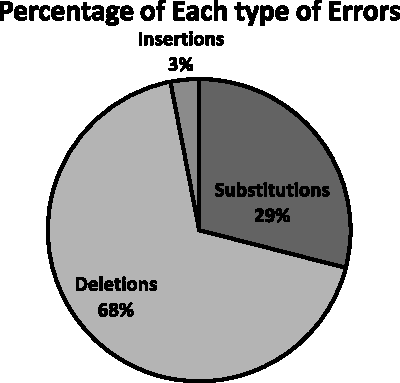
\includegraphics[width=\textwidth]{Figure4.pdf}
\caption{The percentage of each type of error out of the total errors.}
\source{Own Elaboration.}
\label{fig:fig4}
\end{minipage}
\end{figure}

The majority of errors were identified as deletions (68\%), succeeded by
substitutions (29\%), and then insertions (3\%). Upon performing
calculations for substitutions, deletions, and insertions and adding up
the resulting numbers, the sum is divided by the total number of words
in the reference. Then, multiply the resulting number by 100\% to show
that the WER percentage is 38.857\%. \Cref{tbl10} reveals the numbers that
were used in the mathematical equation.

	
\begin{table}[htbp]
\centering
\small
\begin{threeparttable}
\caption{The total sum of the error values categorised by their type with WER percentage.}
\label{tbl10}
\begin{tabular}{@{}
	>{\raggedright\arraybackslash}p{(\columnwidth - 2\tabcolsep) * \real{0.7002}}
	>{\raggedright\arraybackslash}p{(\columnwidth - 2\tabcolsep) * \real{0.2998}}@{}}
\noalign{}
\begin{minipage}[b]{\linewidth}\raggedright
Category
\end{minipage} & 
\begin{minipage}[b]{\linewidth}\raggedright
Number
\end{minipage} \\
\midrule\noalign{}
Deletions (D) & 513 \\
Substitutions (S) & 219 \\
Insertions (I) & 23 \\
Total words in Reference (N) & 1943 \\
Word Error Rate in Percentage (WER) & 38.857\% \\
\bottomrule
\end{tabular}
\source{Own elaboration.}
\end{threeparttable}
\end{table}
	
Regarding deletion errors, the primary cause appears to be the
misidentification of JA affixes, accounting for 55\% of errors. This is
followed by overlapping, where multiple speakers talk simultaneously,
accounting for 26\% of errors. Misrecognising interjections accounted
for 17\% of errors, while deletion of long vowels and shortening length
only accounted for 2\%. \Cref{fig:fig5} shows these percentages in a pie chart.
	
%\begin{figure}[htbp]
%\centering
%\begin{minipage}{0.45\textwidth}
%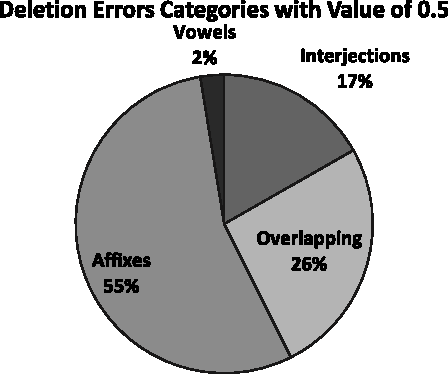
\includegraphics[width=\textwidth]{Figure5.pdf}
%\caption{The percentage of each type of deletion error with 0.5 value.}
%\source{Own Elaboration.}
%\label{fig:fig5}
%\end{minipage}
%\end{figure}

\begin{figure}[h]
\begin{minipage}[t]{0.47\textwidth}
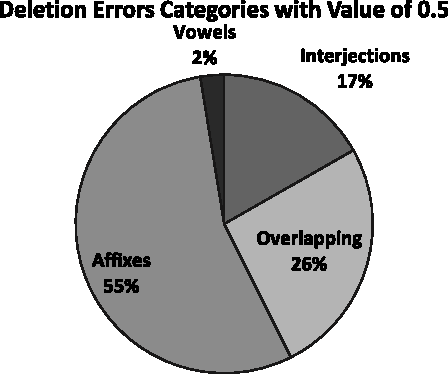
\includegraphics[width=\linewidth]{Figure5.pdf}
\caption{The percentage of each type of deletion error with 0.5 value.}\label{fig:fig5}
\source{Own Elaboration.}
\end{minipage}
\hfill
\begin{minipage}[t]{0.47\textwidth}
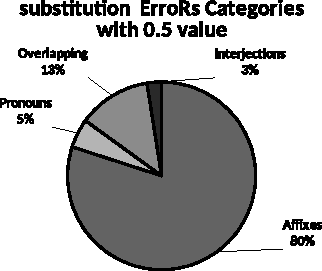
\includegraphics[width=\linewidth]{Figure6.pdf}
\caption{Percentage of each type of substitution error with 0.5 value.}\label{fig:fig6}
\source{Own Elaboration.}
\end{minipage}
\end{figure}

When examining substitution errors, it appears that the primary cause is
the same cause of deletion errors, which is the misidentification of JA
affixes, accounting for 80\% of errors. Overlapping errors account for
12\%, errors with pronouns account for 5\% of errors, while
misrecognised interjections account for 3\%. The percentages are
depicted in a pie chart in \Cref{fig:fig6}.
	
%\begin{figure}[htbp]
%\centering
%\begin{minipage}{0.45\textwidth}
%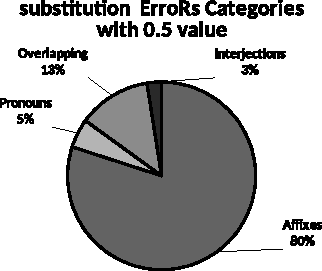
\includegraphics[width=\textwidth]{Figure6.pdf}
%\caption{Percentage of each type of substitution error with 0.5 value.}
%\source{Own Elaboration.}
%\label{fig:fig6}
%\end{minipage}
%\end{figure}

With a total of 8 errors that hold the value of 0.5, the insertion
errors were all caused because of insertion for affixes not found in the
original transcript, as \Cref{fig:fig7} shows.

%\begin{figure}[htbp]
%\centering
%\begin{minipage}{0.45\textwidth}
%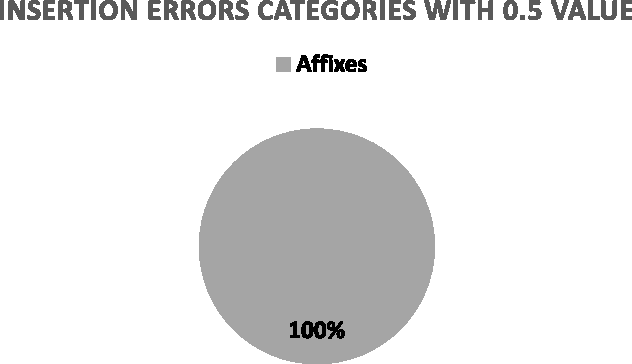
\includegraphics[width=\textwidth]{Figure7.pdf}
%\caption{The percentage of each type of substitution error with 0.5 value.}
%\source{Own Elaboration.}
%\label{fig:fig7}
%\end{minipage}
%\end{figure}

\begin{figure}[h]
\begin{minipage}[t]{0.47\textwidth}
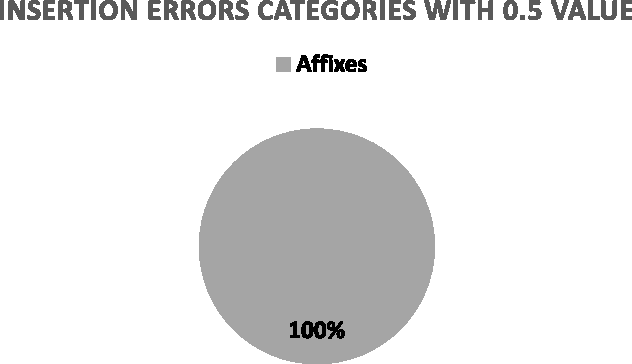
\includegraphics[width=\linewidth]{Figure7.pdf}
\caption{The percentage of each type of substitution error with 0.5 value.}\label{fig:fig7}
\source{Own Elaboration.}
\end{minipage}
\hfill
\begin{minipage}[t]{0.47\textwidth}
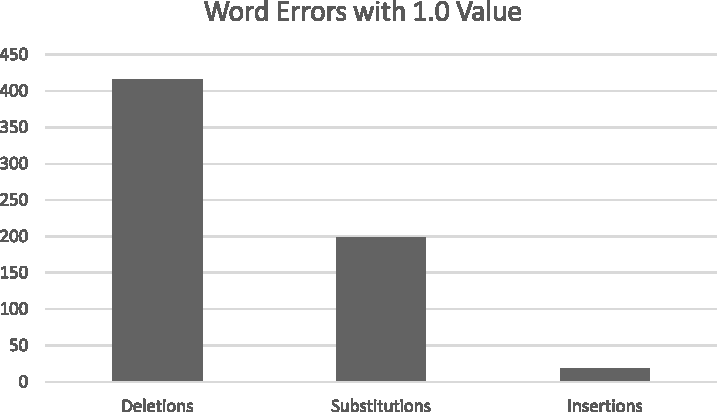
\includegraphics[width=\linewidth]{Figure8.pdf}
\caption{The Total number of errors for each type with a 1.0 value.}\label{fig:fig8}
\source{Own Elaboration.}
\end{minipage}
\end{figure}


On the other hand, the analysis of word errors that hold a 1.0 value
revealed that 416 of these errors were deletions, followed by
substitutions with 199 errors, while insertions were only 19 errors.
\Cref{fig:fig8} shows a clustered column chart that compares the values across
these categories.

%\begin{figure}[htbp]
%\centering
%\begin{minipage}{.45\textwidth}
%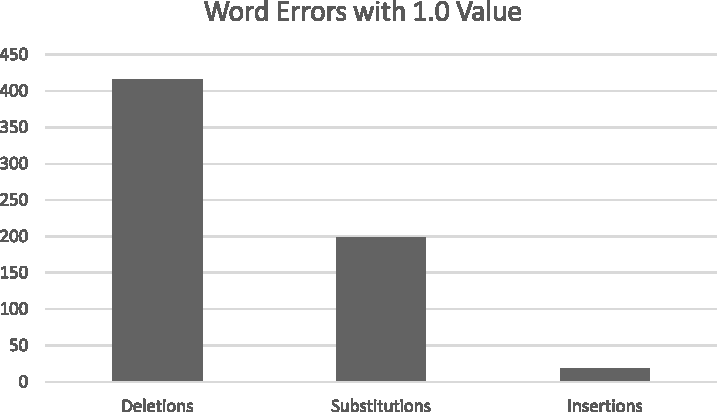
\includegraphics[width=\textwidth]{Figure8.pdf}
%\caption{The Total number of errors for each type with a 1.0 value.}
%\source{Own Elaboration.}
%\label{fig:fig8}
%\end{minipage}
%\end{figure}


\section{Conclusion}\label{sec-conclusion}

This research paper examines the linguistic accuracy of veed.io when
automatically generating intralingual subtitles for a video in Jordanian
Arabic, where two female broadcasters talk about the etiquette of meals
in Ramadan. In specific, it explores the obstacles that machines may
face when dealing with various linguistic and phonetic phenomena in
Jordanian Arabic.

In the qualitative part, errors are categorised into three main types:
deletions, substitutions, and insertions. Deletions occur when the
system does not fully or partially transcribe the utterance,
substitution happens when the system replaces one utterance with
another, and insertion occurs when the system inserts an item that does
not exist in the original utterance. Furthermore, the analysis
subcategorises errors into two main types. Errors that did not
significantly affect the comprehension of the text are assigned a value
of 0.5, and errors that affected the comprehension of the subtitles are
assigned a value of 1.0.

Notably, the analysis revealed the deletion of 0.5 errors involves
affixes, interjections, overlapping, and vowel length, while those of
1.0 include nouns, verbs, function words, and foreign words. Similarly,
substitution errors of 0.5 are affixes, interjections, overlapping, and
pronouns, while those of 1.0 errors are nouns, verbs, function words,
and foreign words. Lastly, insertion errors of 0.5 are affixes, while
those of 1.0 are nouns, verbs, and function words. These findings have
implications for the readability of the comprehension of subtitles.

In the quantitative analysis, the study employed Excel formulas to
calculate the word error rate (WER), which amounted to 38.857\%, showing
that the majority of errors are identified as deletions (68\%),
succeeded by substitutions (29\%), and finally insertions (3\%).

Furthermore, the research methodology proved to be effective in
suggesting a specific classification for AI-Powered subtitles and
analysing the errors. The proposed taxonomy categorises AI-powered
subtitles into intralingual and interlingual types based on two factors:
the used technology and the target language. The study suggests that
Intralingual subtitles can be subcategorised into four main types:
SR-based; ASR-based; Semi-ASR-based; SLR-based, and interlingual
subtitles can be MT-based or Semi MT-based. Moreover, the methodology
was developed with consideration for the unique orthographical rules and
writing system of the Arabic language.

To acknowledge the limitations of our study, measuring ASR accuracy is
necessary and requires tools that are specifically designed for the
Arabic language. These tools should be able to differentiate between two
types of errors, which can be 0.5 error or 1.0 error, along with no
errors that hold a value of 0. Due to the lack of such a tool, the study
used Excel formulas and manually differentiated between these errors.
Also, more research is needed in the field of Jordanian dialect.

Based on the findings, the study suggests more research in the field of
ASR systems when dealing with different Arabic dialects and the other
types of technology that deal with language. Also, subtitlers and
content creators should be aware of these challenges when using these
online tools.

This research serves as a steppingstone towards development in language
technology. By continuing to investigate and expand our knowledge, we
can contribute to advancements and improvements in auto-generated
subtitles of Jordanian Arabic and make meaningful contributions to AVT
and NLP.

\section*{Acknowledgment}
	
The authors are thankful to the Deanship of Graduate Studies and Scientific Research at University of Bisha for supporting this work through the Fast-Track Research Support Program.
	

\printbibliography\label{sec-bib}
	
	
%full list: conceptualization,datacuration,formalanalysis,funding,investigation,methodology,projadm,resources,software,supervision,validation,visualization,writing,review
\begin{contributors}[sec-contributors]
	\authorcontribution{Wala’ Mohammad Akasheh}[conceptualization,datacuration,formalanalysis,methodology,investigation,validation,writing,review,visualization]
	
	\authorcontribution{Ahmad S. Haider}[conceptualization,datacuration,formalanalysis,investigation,methodology,supervision,validation,review,visualization]
	
	\authorcontribution{Bassam Al-Saideen}[investigation,resources,review]
	
	\authorcontribution{Yousef Sahari}[conceptualization,resources,review]
\end{contributors}
	
	
\end{document}
                                                                                          